\documentclass[letterpaper, 11pt]{report}
% This is the project summary of the final project for Computer Science 20 at
% Western Canada High School by Zhantong Zhang in the December of 2013.

\usepackage[top=1in, bottom=1in, left=1in, right=1in]{geometry}
\usepackage[final]{pdfpages}
\usepackage{listings}
\usepackage{color}
\usepackage{ifthen}
\usepackage{fancyref}
\usepackage{makeidx}
\usepackage[hidelinks,bookmarks,pdfpagelabels,breaklinks=true]{hyperref}
\def\UrlBreaks{\do\A\do\B\do\C\do\D\do\E\do\F\do\G\do\H\do\I\do\J
\do\K\do\L\do\M\do\N\do\O\do\P\do\Q\do\R\do\S\do\T\do\U\do\V
\do\W\do\X\do\Y\do\Z\do\[\do\\\do\]\do\^\do\_\do\`\do\a\do\b
\do\c\do\d\do\e\do\f\do\g\do\h\do\i\do\j\do\k\do\l\do\m\do\n
\do\o\do\p\do\q\do\r\do\s\do\t\do\u\do\v\do\w\do\x\do\y\do\z
\do\.\do\@\do\\\do\/\do\!\do\_\do\|\do\;\do\>\do\]\do\)\do\,
\do\?\do\'\do\+\do\=\do-\do\#}

\newcommand{\entityintro}[3]{%
  \hbox to \hsize{%
    \vbox{%
      \hbox to .2in{}%
    }%
    {\bf  #1}%
    \dotfill\pageref{#2}%
  }
  \makebox[\hsize]{%
    \parbox{.4in}{}%
    \parbox[l]{5in}{%
      \vspace{1mm}%
      #3%
      \vspace{1mm}%
    }%
  }%
}
\newcommand{\refdefined}[1]{
\expandafter\ifx\csname r@#1\endcsname\relax
\relax\else
{$($in \ref{#1}, page \pageref{#1}$)$}\fi}
\chardef\textbackslash=`\\

% flowchart elements
\usepackage{tikz}
\usetikzlibrary{shapes.geometric, arrows}
\tikzstyle{startstop} = [rectangle, rounded corners, minimum width=3cm, minimum
height=1cm,text centered, draw=black, fill=red!30]
\tikzstyle{io} = [trapezium,
trapezium left angle=70, trapezium right angle=110, minimum width=2.5cm, minimum
height=1cm, text centered, draw=black, fill=blue!30, text width=3cm]
\tikzstyle{process} =
[rectangle, minimum width=3cm, minimum height=1cm, text centered, draw=black,
fill=orange!30, text width=3cm]
\tikzstyle{decision} = [diamond, minimum width=3cm, minimum
height=1cm, text centered, draw=black, fill=green!30, text width=3cm]
\tikzstyle{arrow} =
[thick,->,>=stealth]

\usepackage{graphicx}
\DeclareGraphicsExtensions{.pdf,.png,.jpg}
\usepackage{caption}
\usepackage{subcaption}

\usepackage{titlesec}
\titleformat{\chapter}[frame]{\normalfont\huge\bfseries}{\chaptertitlename\
\thechapter}{20pt}{\huge}
%\titleformat{\section}{\normalfont\bfseries}{\thesection}{-5pt}{}
% \titleformat{\subsection}{\normalfont\bfseries}{}{0pt}{\large}

\begin{document}
\newcommand{\HRule}{\rule{\linewidth}{0.5mm}}
\begin{titlepage}
\begin{center}
\textsc{\LARGE Computer Science 20}\\[1cm]
\textsc{\Large Final Project}\\[1cm]

% Title
\HRule \\[0.2cm]
{\huge\bfseries Person of Interest \\[0.2cm] }
\HRule \\[1cm]

% Author

\begin{tabular}{cc}
\Large Zhantong & \Large \textsc{Zhang}\\
(Tony) &
\end{tabular}

\vfill

% Bottom of the page
{\large Janurary 9, 2013\par
Western Canada High School
}
\end{center}
\end{titlepage}
\chapter*{LICENSE}
\label{chap:LICENSE}
\thispagestyle{empty}
{\ttfamily\raggedright
Copyright (c) 2013, Zhantong ZHANG \\
All rights reserved. \\
\vspace{1\baselineskip}\vspace{-\parskip}
Redistribution and use in source and binary forms, with or without \\
modification, are permitted provided that the following conditions are met: \\
\vspace{1\baselineskip}\vspace{-\parskip}
\ \* Redistributions of source code must retain the above copyright notice, \\
   this list of conditions and the following disclaimer. \\
\ \* Redistributions in binary form must reproduce the above copyright \\
   notice, this list of conditions and the following disclaimer in the \\
   documentation and/or other materials provided with the distribution. \\
\ \* Neither the name of Person of Interest nor the names of its contributors \\
   may be used to endorse or promote products derived from this software \\
   without specific prior written permission. \\
\vspace{1\baselineskip}\vspace{-\parskip}
THIS SOFTWARE IS PROVIDED BY THE COPYRIGHT HOLDERS AND CONTRIBUTORS "AS IS" \\
AND ANY EXPRESS OR IMPLIED WARRANTIES, INCLUDING, BUT NOT LIMITED TO, THE \\
IMPLIED WARRANTIES OF MERCHANTABILITY AND FITNESS FOR A PARTICULAR PURPOSE \\
ARE DISCLAIMED. IN NO EVENT SHALL THE COPYRIGHT OWNER OR CONTRIBUTORS BE \\
LIABLE FOR ANY DIRECT, INDIRECT, INCIDENTAL, SPECIAL, EXEMPLARY, OR \\
CONSEQUENTIAL DAMAGES (INCLUDING, BUT NOT LIMITED TO, PROCUREMENT OF \\
SUBSTITUTE GOODS OR SERVICES; LOSS OF USE, DATA, OR PROFITS; OR BUSINESS \\
INTERRUPTION) HOWEVER CAUSED AND ON ANY THEORY OF LIABILITY, WHETHER IN \\
CONTRACT, STRICT LIABILITY, OR TORT (INCLUDING NEGLIGENCE OR OTHERWISE) \\
ARISING IN ANY WAY OUT OF THE USE OF THIS SOFTWARE, EVEN IF ADVISED OF THE \\
POSSIBILITY OF SUCH DAMAGE. \\
THIS WORK IS A WORK FOR AN ACADEMIC COURSE, HOWEVER, IT IS NOT INTENDED FOR \\
ACTIONS OF PLAGIARISM. PLAGIARISM IS A SERIOUS OFFENCE THAT VIOLATES BOTH \\
ACADEMIC AND PERSONAL INTEGRITY AND MAY CAUSE SERIOUS CONSEQUENCES IN YOUR \\
INSTITUTION. \\
THIS LICENSE DOES NOT APPLY TO PROGRAM RESOURCES. LOCATION DESCRIPTIONS ARE \\
ADAPTED FROM RELATED ARTICLES IN WIKIPEDIA. CC-BY-SA 3.0 LICENSE THAT CAN \\
BE OBTAINED FROM \url{HTTP://GOO.GL/gh86uJ} APPLIES TO THOSE RESOURCES.
}
\addtocounter{page}{-1}
\setcounter{tocdepth}{2}

\tableofcontents

% proposal copy
\part{Copy of the Project Proposal}
The original signed proposal is attached in the binder; the following is a
\emph{copy} of the proposal:

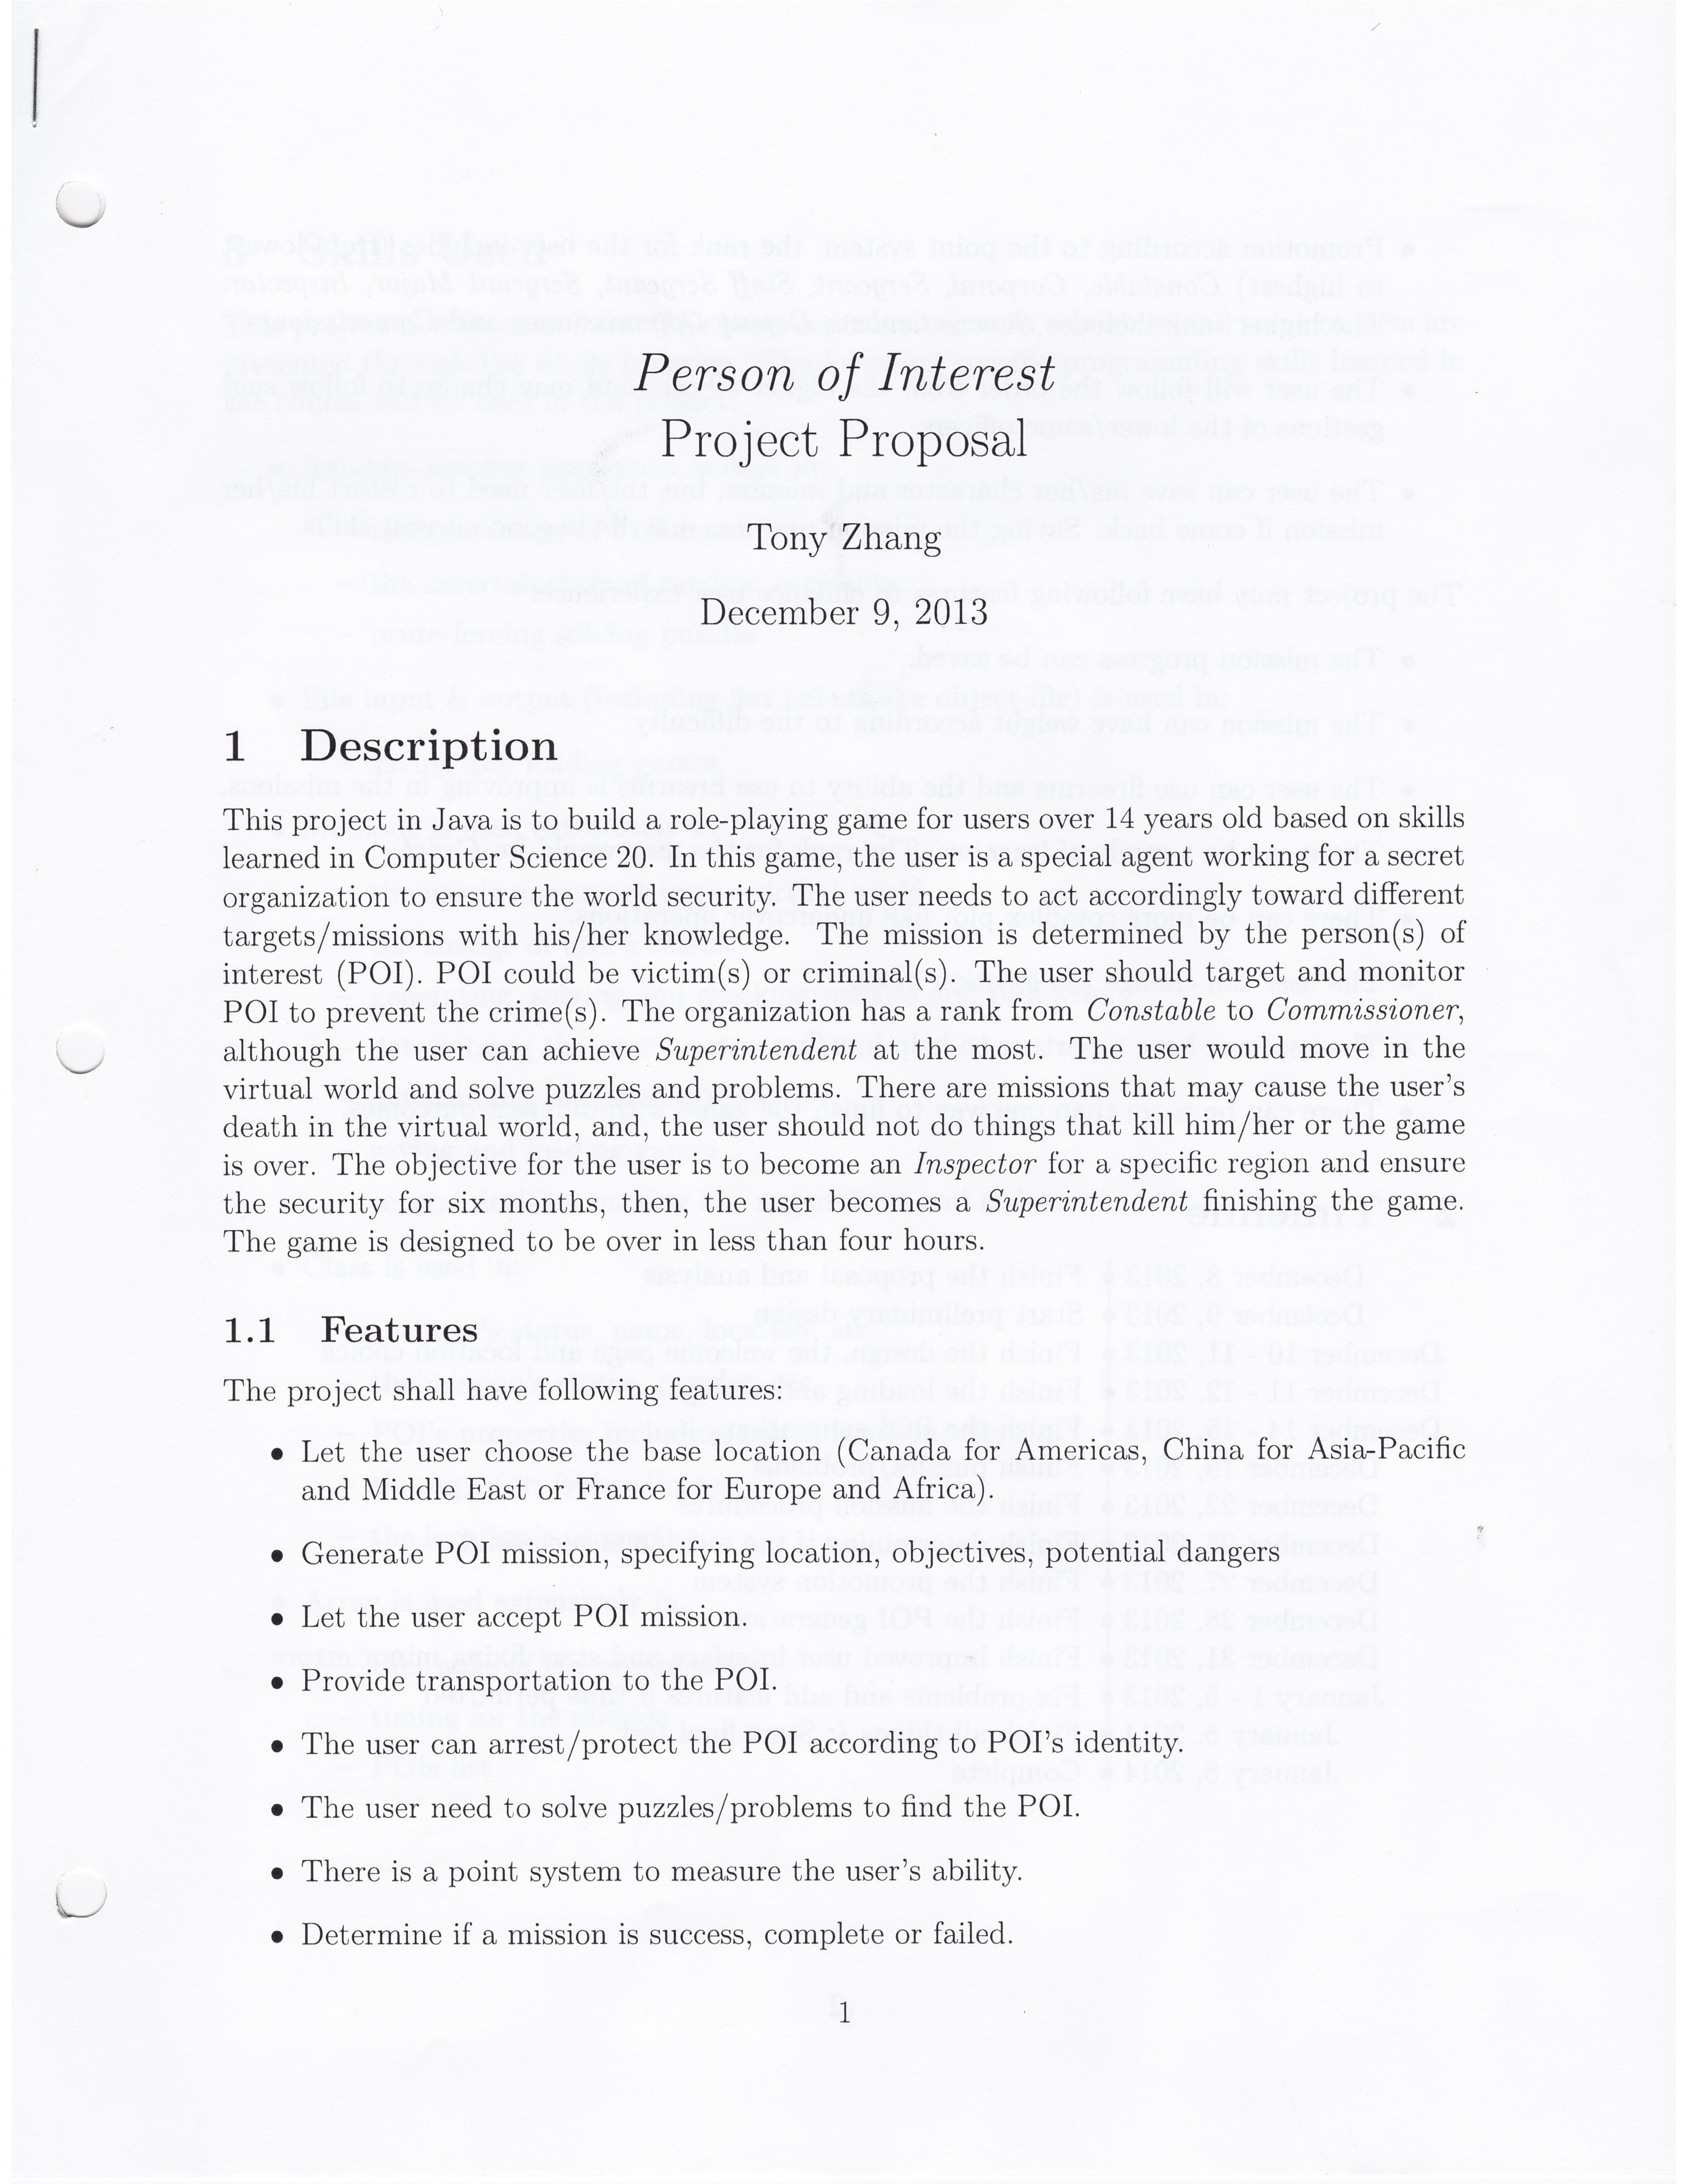
\includegraphics[width=0.9\linewidth]{./img/prop-1}

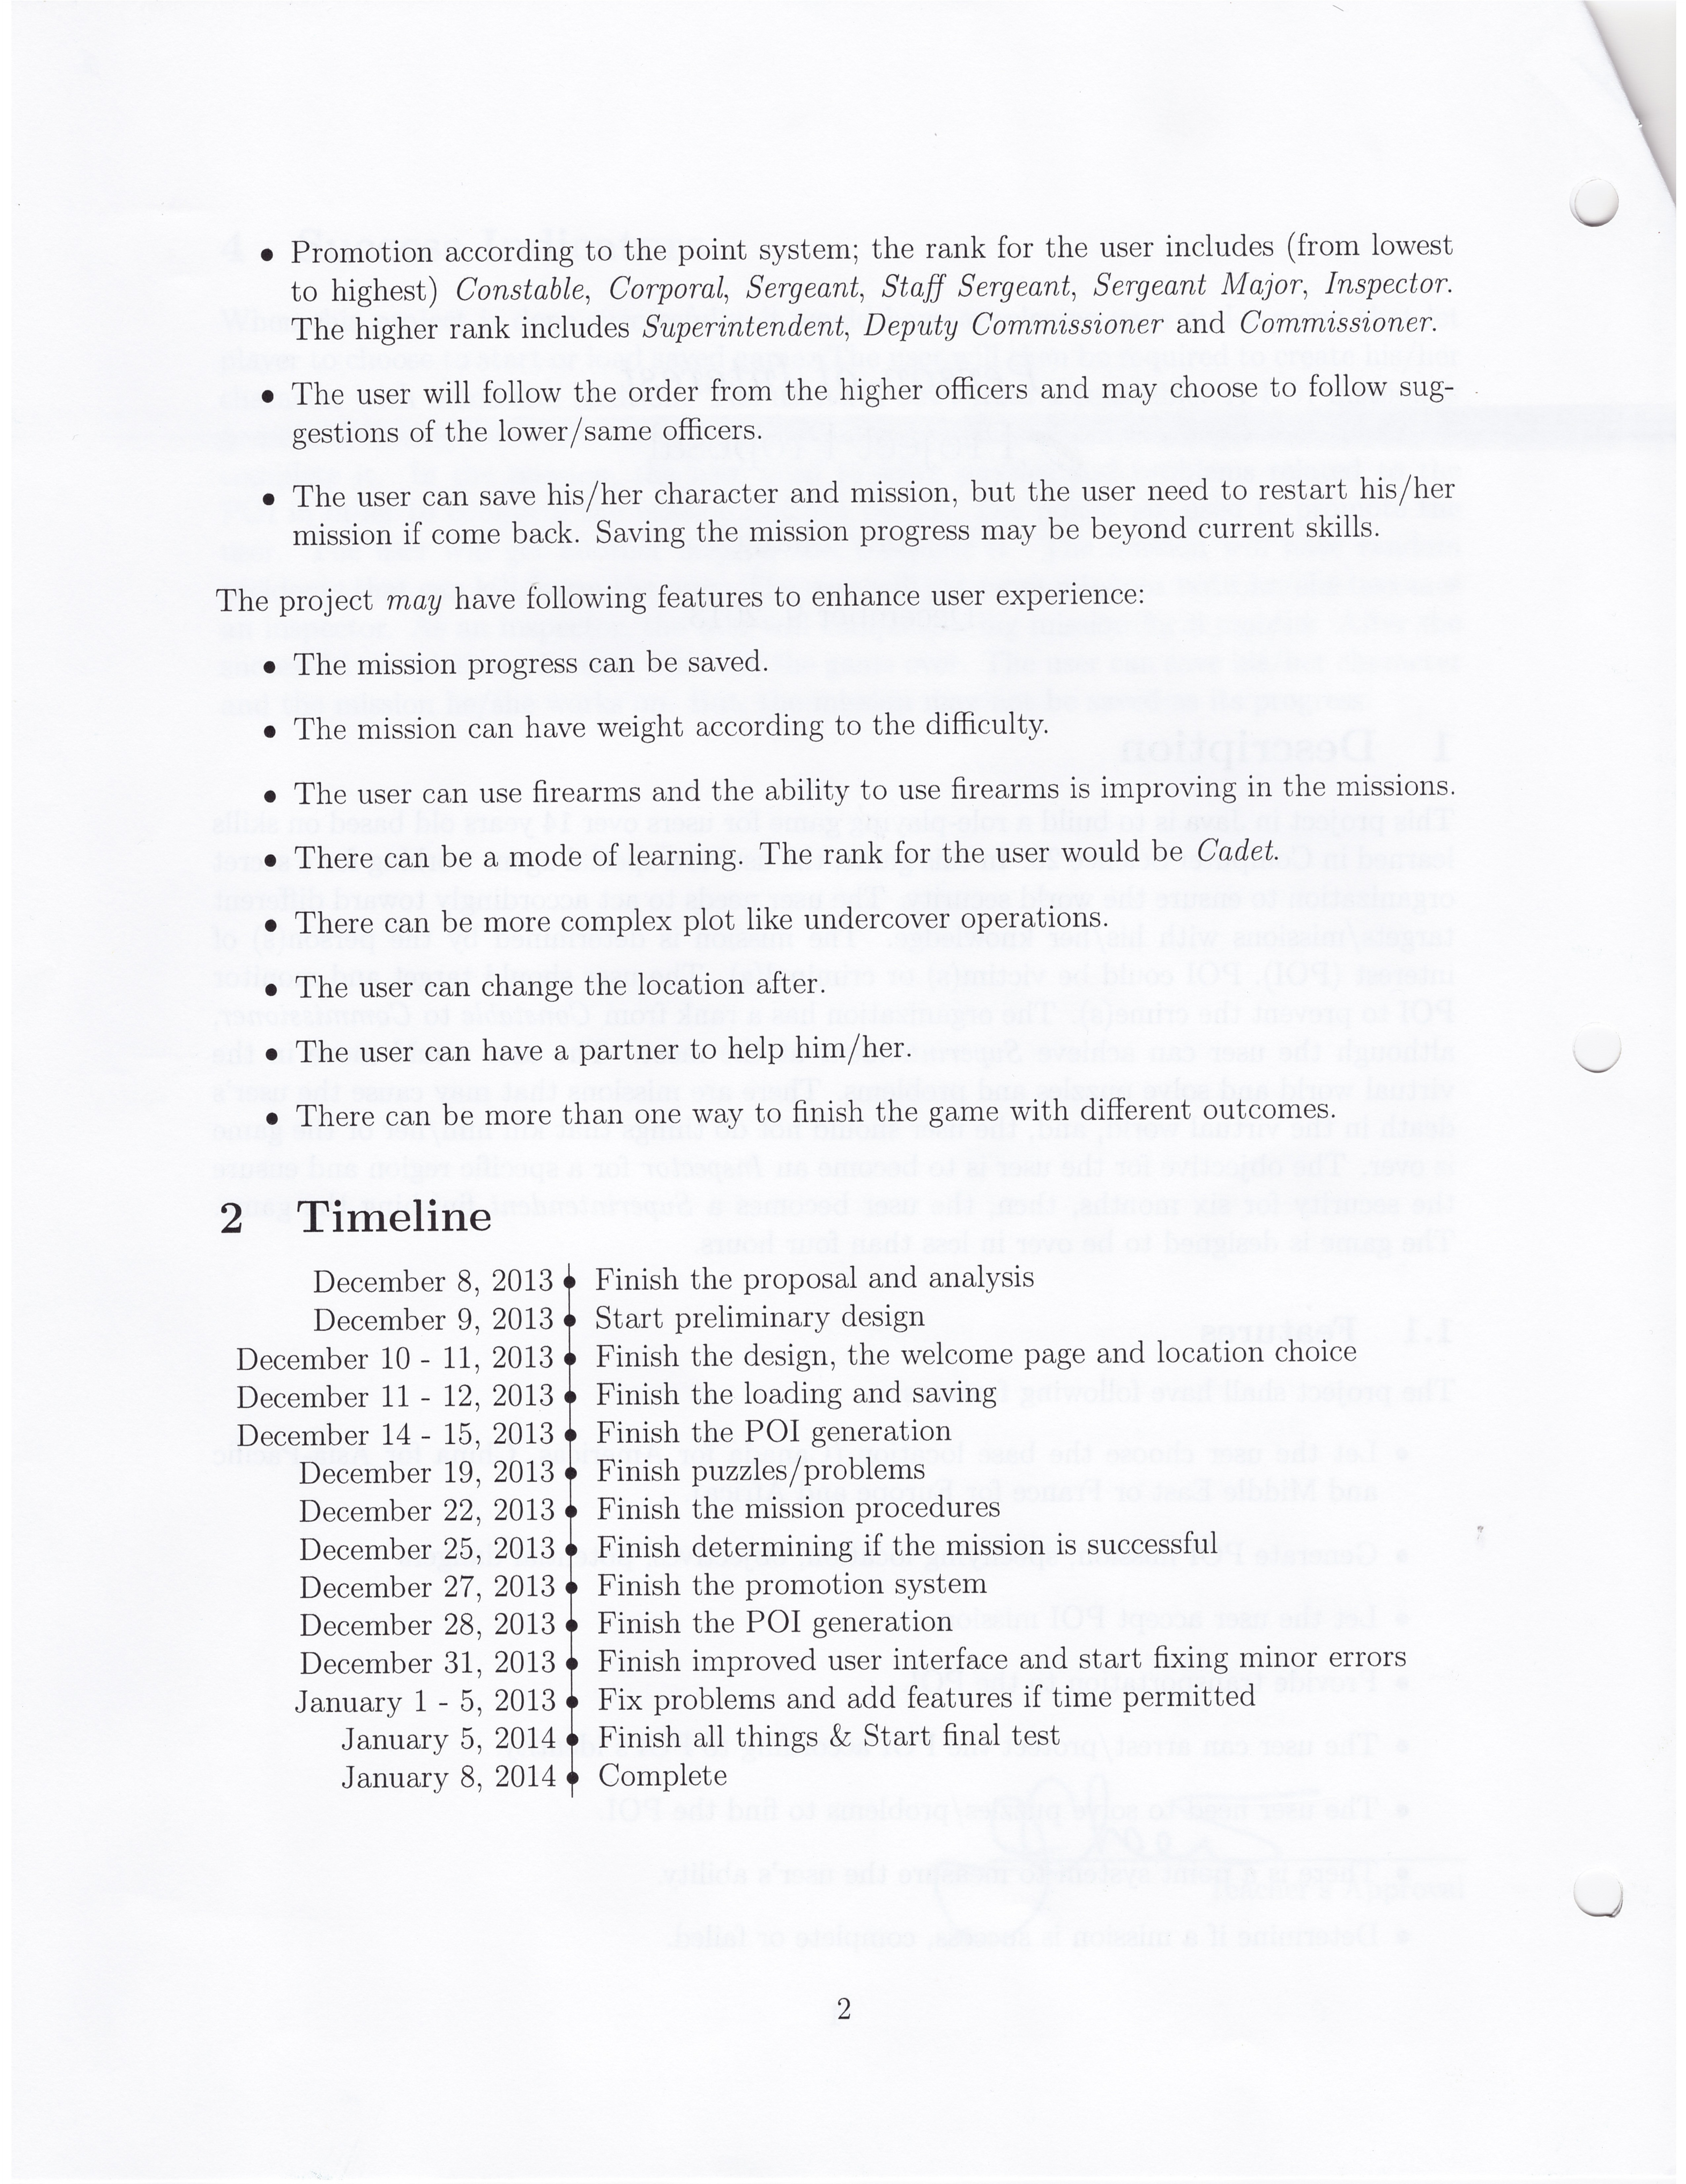
\includegraphics[width=0.9\linewidth]{./img/prop-2}

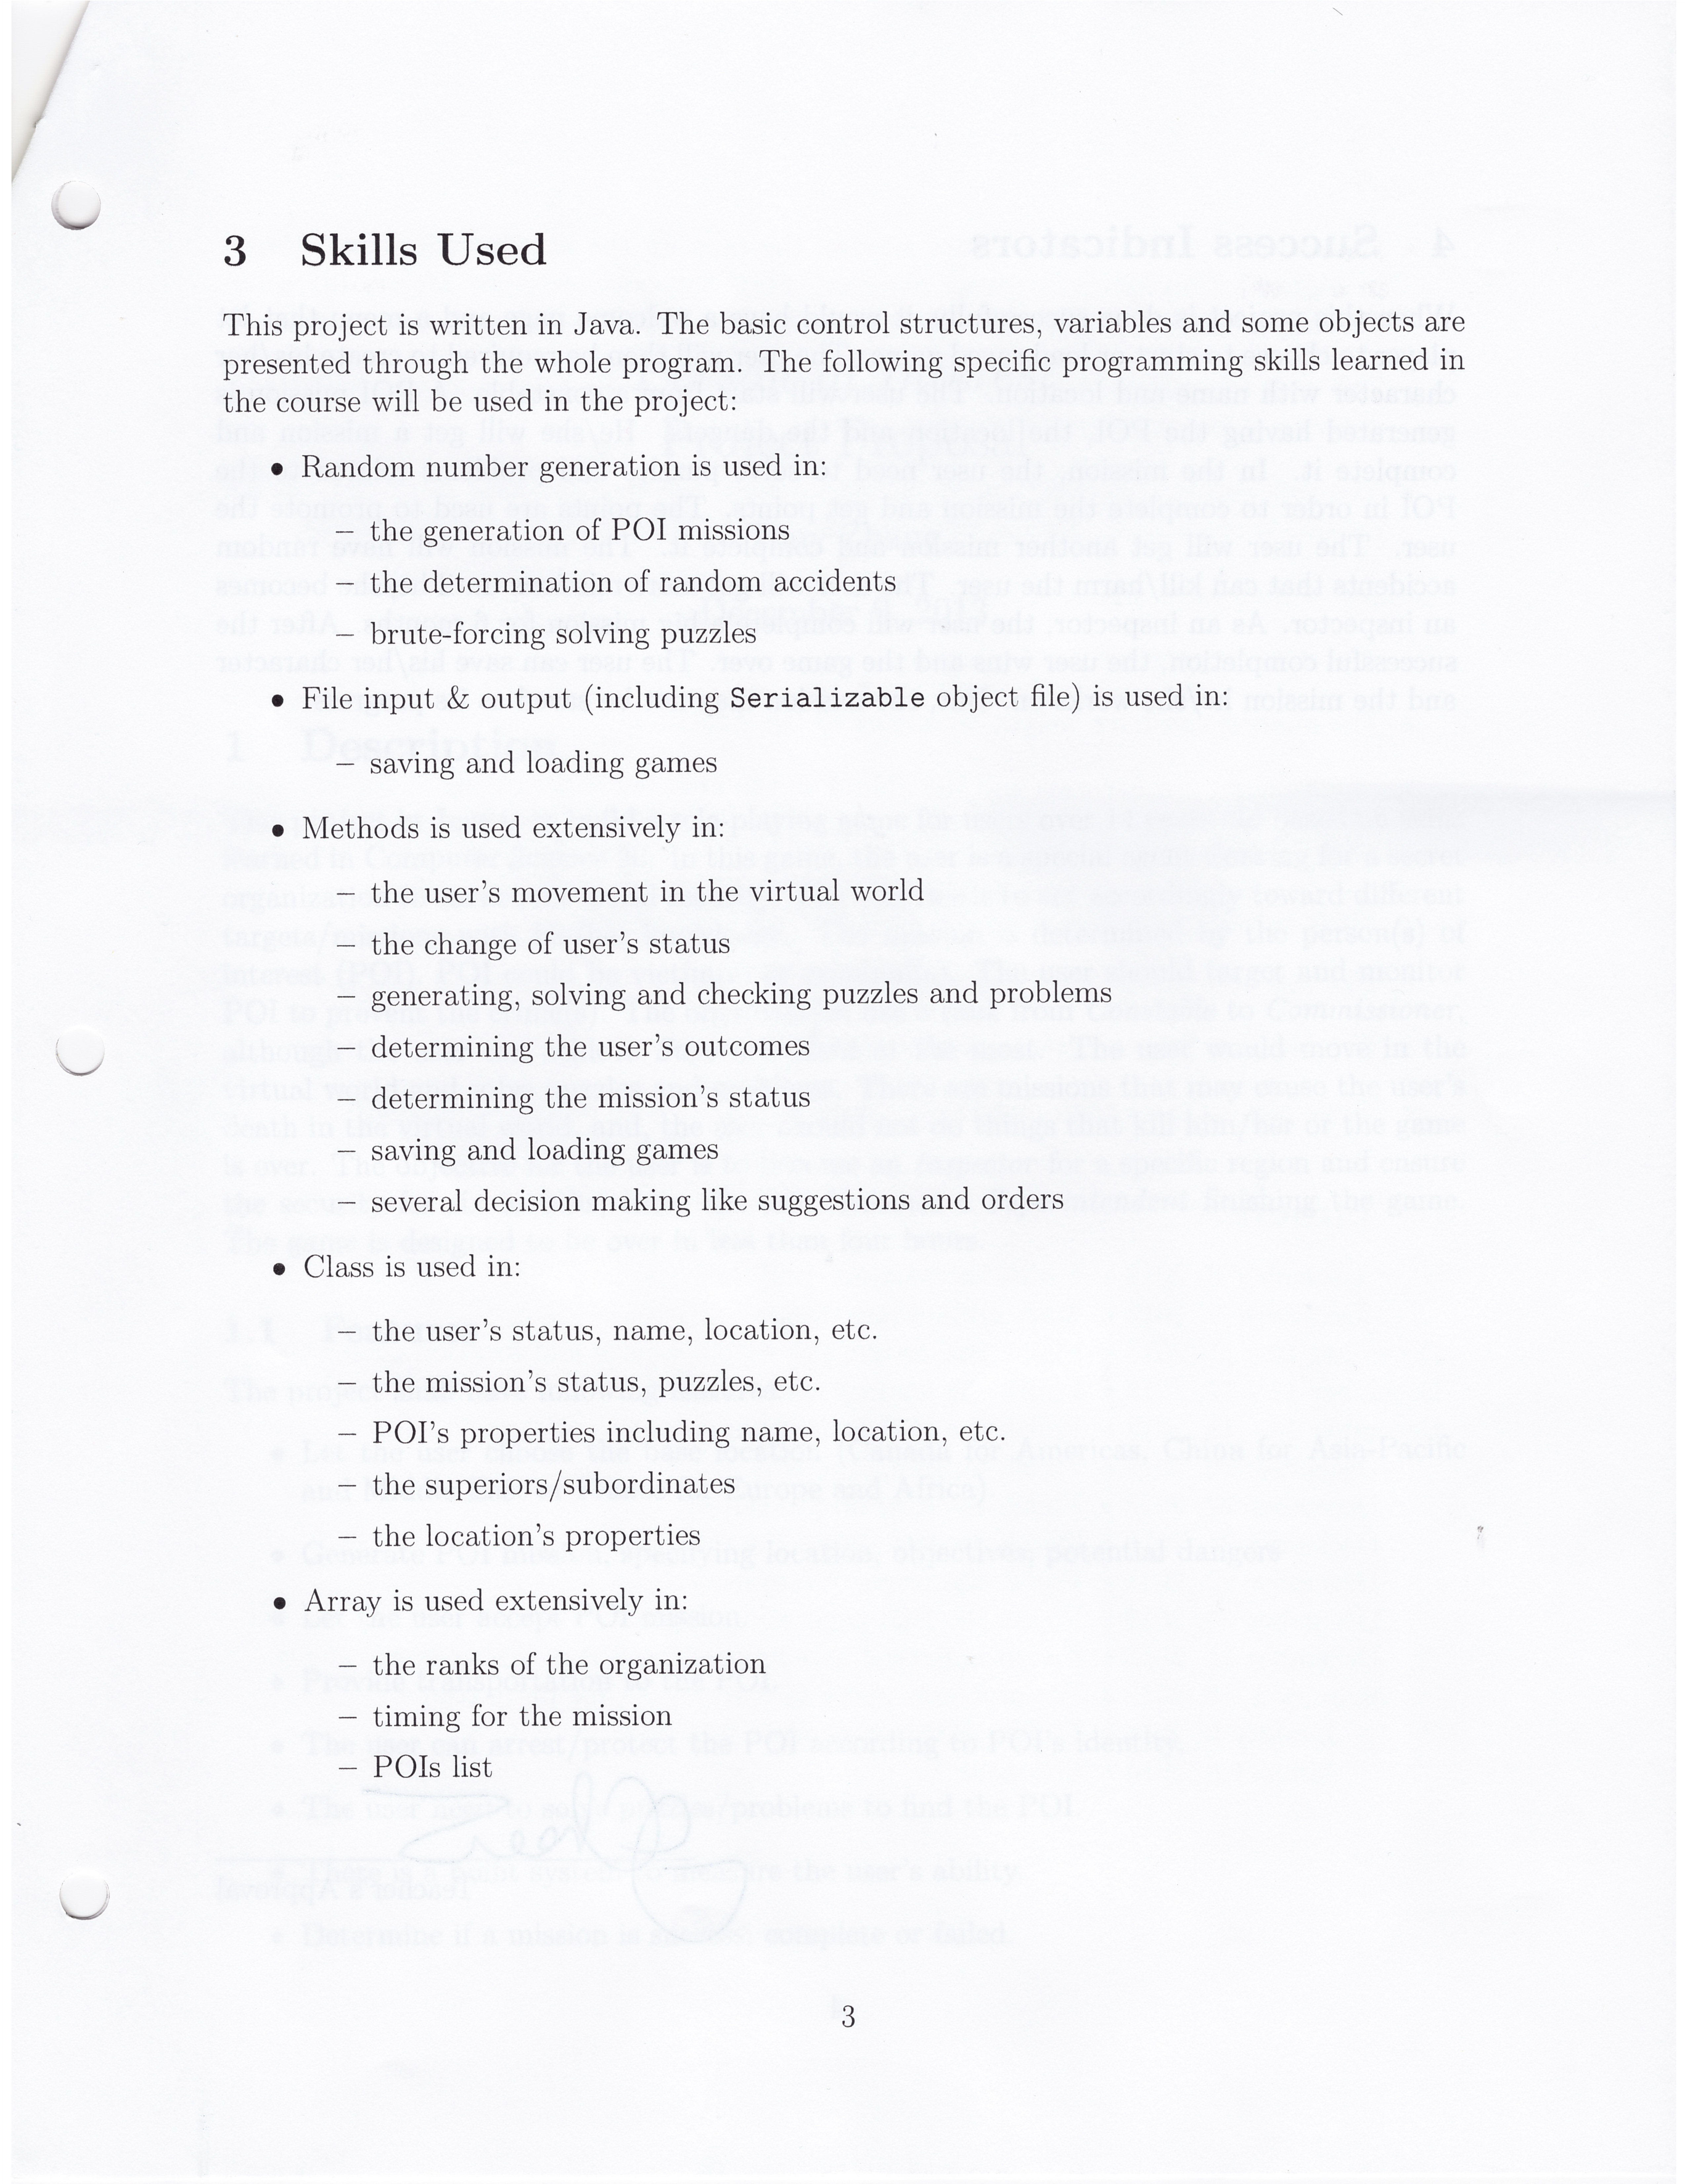
\includegraphics[width=0.9\linewidth]{./img/prop-3}


\includegraphics[width=0.9\linewidth]{./img/prop-4}

% design
\part{Preliminary Design}
\chapter{Diagrams}
% flowchart
\section{Program Process}
\subsection{Overall Process}
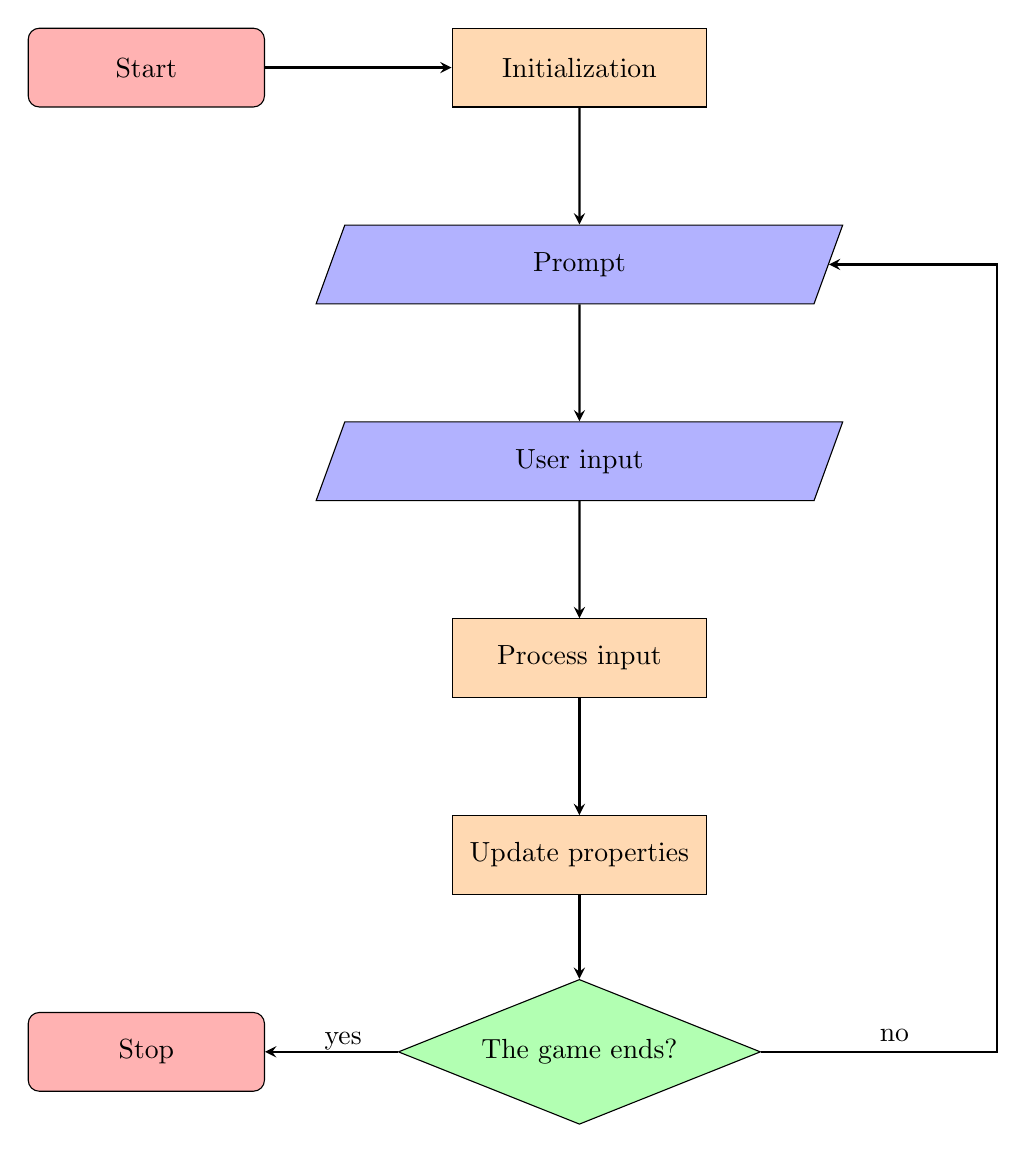
\begin{tikzpicture}[node distance=2.5cm]

\node(start)[startstop]{Start};
\node(init)[process, right of=start, xshift=3cm]{Initialization};
\node(prompt)[io, below of=init]{Prompt};
\node(in1)[io, below of=prompt]{User input};
\node(procInput)[process, below of=in1]{Process input};
\node(update)[process, below of=procInput]{Update properties};
\node(ifQuit)[decision, below of=update, aspect=2.5]{The game ends?};
\node(stop)[startstop, left of=ifQuit, xshift=-3cm]{Stop};

\draw[arrow](start) -- (init);
\draw[arrow](init) -- (prompt);
\draw[arrow](prompt) -- (in1);
\draw[arrow](in1) -- (procInput);
\draw[arrow](procInput) -- (update);
\draw[arrow](update) -- (ifQuit);
\draw[arrow](ifQuit) node[anchor=south, xshift=4cm]{no} --
([xshift=3cm]ifQuit.east) |- (prompt);
\draw[arrow](ifQuit) node[anchor=south, xshift=-3cm, yshift=-0.1cm]{yes} --
(stop);

\end{tikzpicture}

\subsection{Initialization}
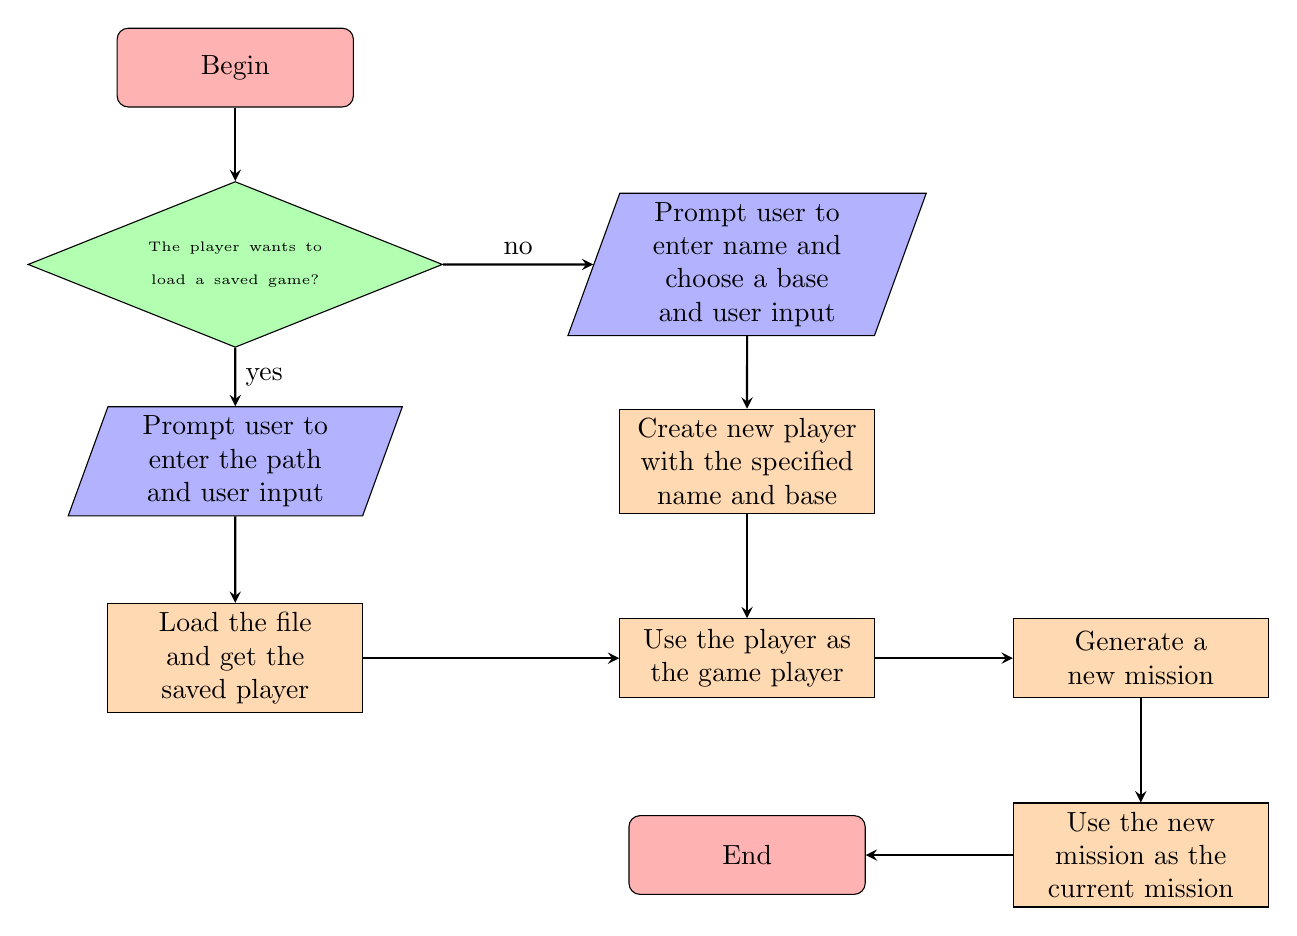
\begin{tikzpicture}[node distance=2.5cm]

\node(begin)[startstop]{Begin};
\node(ifLoad)[decision, below of=begin, aspect=2.5, text width=3cm]{\tiny{The
player wants to load a saved game?}};

\node(loadPath)[io, below of=ifLoad, text width=3cm]{Prompt user to enter the
path and user input};
\node(load)[process, below of=loadPath]{Load the file and get
the saved player};

\node(new)[io, right of=ifLoad, xshift=4cm]{Prompt user
to enter name and choose a base and user input};
\node(newPlayer)[process, below of=new]{Create new player
with the specified name and base};

\node(player)[process, below of=newPlayer]{Use the player as the
game player};
\node(newMst)[process, right of=player, xshift=2.5cm]{Generate a new
mission};
\node(mst)[process, below of=newMst]{Use the new mission as
the current mission};
\node(end)[startstop, left of=mst, xshift=-2.5cm]{End};

\draw[arrow](begin) --(ifLoad);
\draw[arrow](ifLoad) -- node[anchor=west]{yes}(loadPath);
\draw[arrow](ifLoad) -- node[anchor=south]{no}(new);

\draw[arrow](loadPath) -- (load);

\draw[arrow](new) --  (newPlayer);

\draw[arrow](load) -- (player);
\draw[arrow](newPlayer) -- (player);
\draw[arrow](player) -- (newMst);
\draw[arrow](newMst) -- (mst);
\draw[arrow](mst) -- (end);

\end{tikzpicture}

\subsection{Prompt}
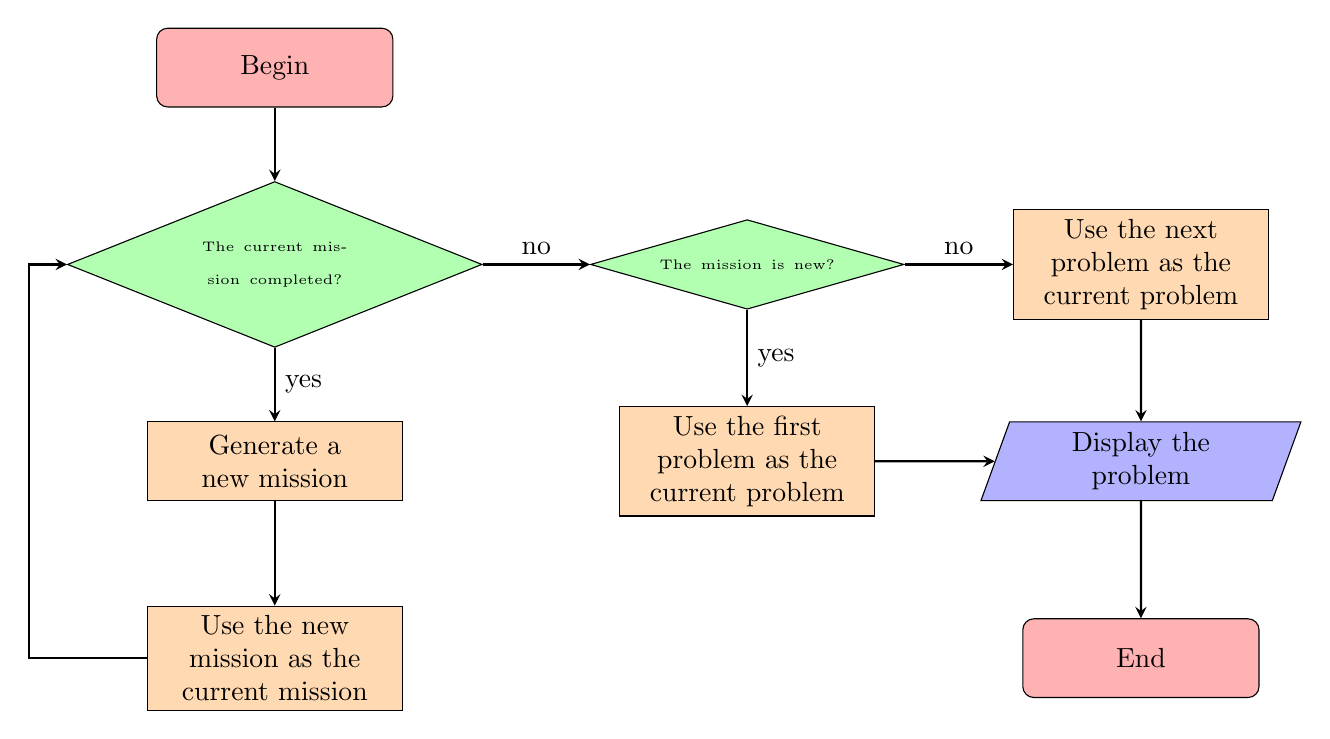
\begin{tikzpicture}[node distance=2.5cm]

\node(begin)[startstop]{Begin};
\node(ifComp)[decision, below of=begin, aspect=2.5]{\tiny{The current mission
completed?}};

\node(generate)[process, below of=ifComp]{Generate a new
mission};
\node(use)[process, below of=generate]{Use the new mission as
the current mission};

\node(ifNew)[decision, right of=ifComp, text width=2.5cm,
xshift=3.5cm, aspect=3.5]{\tiny{The mission is new?}};
\node(nextProb)[process, right of=ifNew, xshift=2.5cm]{Use the next problem as
the current problem};
\node(1stProb)[process, below of=ifNew]{Use the first problem as the current
problem};
\node(disp)[io, below of=nextProb]{Display the problem};
\node(end)[startstop, below of=disp]{End};

\draw[arrow](begin) -- (ifComp);
\draw[arrow](ifComp) -- node[anchor=west]{yes}(generate);
\draw[arrow](generate) -- (use);
\draw[arrow](use) -- ([xshift=-1.5cm]use.west) |- (ifComp);

\draw[arrow](ifComp) -- node[anchor=south]{no}(ifNew);
\draw[arrow](ifNew) -- node[anchor=south]{no}(nextProb);
\draw[arrow](ifNew) -- node[anchor=west]{yes}(1stProb);
\draw[arrow](1stProb) -- (disp);
\draw[arrow](nextProb) -- (disp);
\draw[arrow](disp) -- (end);

\end{tikzpicture}

\subsection{User Input}
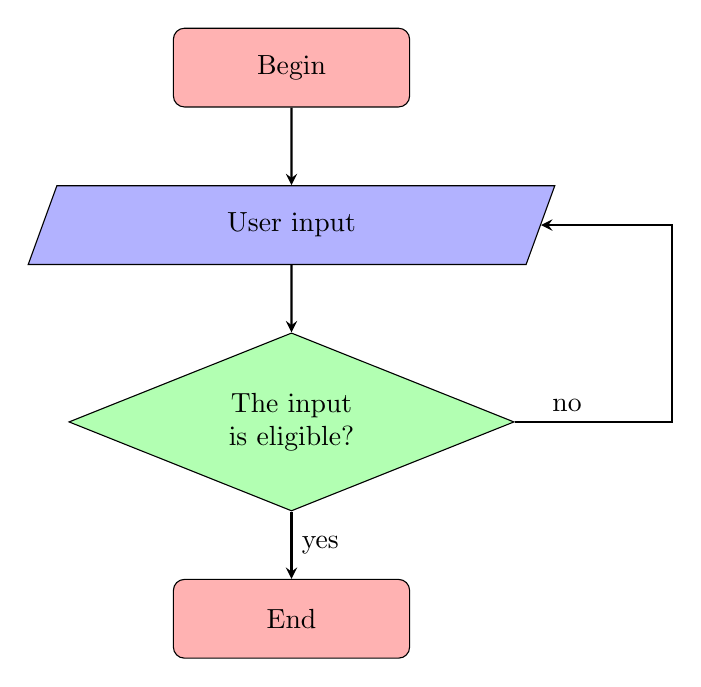
\begin{tikzpicture}[node distance=2.5cm]

\node(begin)[startstop]{Begin};
\node(in)[io, below of=begin, yshift=0.5cm]{User input};
\node(trap)[decision, below of=in, aspect=2.5]{The input is eligible?};
\node(end)[startstop, below of=trap]{End};

\draw[arrow](begin) -- (in);
\draw[arrow](in) -- (trap);
\draw[arrow](trap) node[anchor=south, xshift=3.5cm]{no} --
([xshift=2cm]trap.east) |- (in);
\draw[arrow](trap) -- node[anchor=west]{yes}(end);

\end{tikzpicture}
\subsubsection{Determine if the input is eligible for commands}
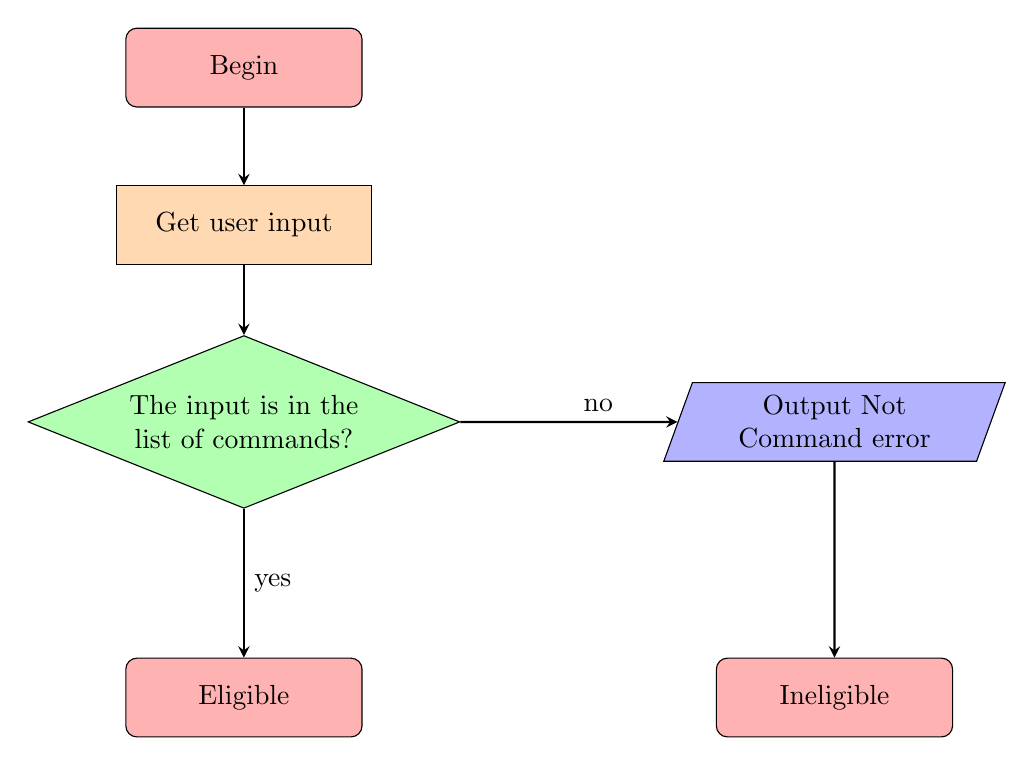
\begin{tikzpicture}[node distance=2.5cm]

\node(begin)[startstop]{Begin};
\node(in)[process, below of=begin, yshift=0.5cm]{Get user input};
\node(trap)[decision, below of=in, aspect=2.5]{The input is in the list of
commands?};
\node(error)[io, right of=trap, xshift=5cm]{Output Not Command error};
\node(good)[startstop, below of=trap, yshift=-1cm]{Eligible};
\node(bad)[startstop, right of=good, xshift=5cm]{Ineligible};

\draw[arrow](begin) -- (in);
\draw[arrow](in) -- (trap);
\draw[arrow](trap) -- node[anchor=west]{yes}(good);
\draw[arrow](trap) node[anchor=south, xshift=4.5cm]{no} --
(error);
\draw[arrow](error) -- (bad);

\end{tikzpicture}

\subsubsection{Determine if the input is eligible for integers in a specific
range}
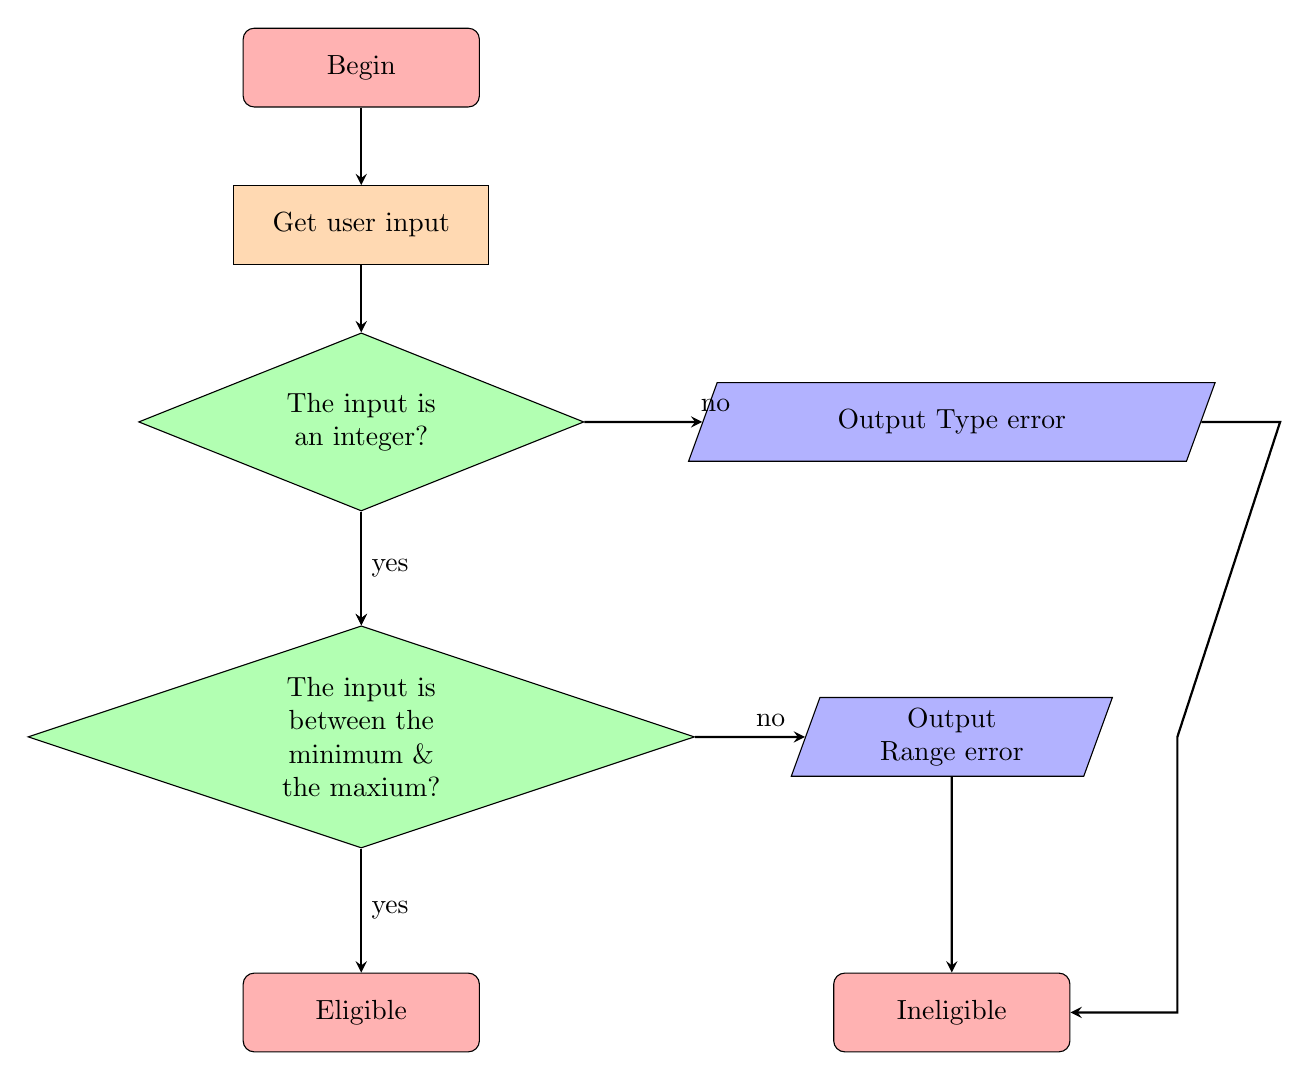
\begin{tikzpicture}[node distance=2.5cm]

\node(begin)[startstop]{Begin};
\node(in)[process, below of=begin, yshift=0.5cm]{Get user input};
\node(trap)[decision, below of=in, aspect=2.5]{The input is an integer?};
\node(maxMin)[decision, below of=in, aspect=3, below of=trap, yshift=1cm]{The input is between the minimum \& the
maxium?};
\node(errorType)[io, right of=trap, xshift=5cm]{Output Type error};
\node(errorRange)[io, right of=maxMin, xshift=5cm]{Output Range error};
\node(good)[startstop, below of=maxMin, yshift=-1cm]{Eligible};
\node(bad)[startstop, right of=good, xshift=5cm]{Ineligible};

\draw[arrow](begin) -- (in);
\draw[arrow](in) -- (trap);
\draw[arrow](trap) -- (maxMin);
\draw[arrow](trap) -- node[anchor=west]{yes}(maxMin);
\draw[arrow](maxMin) -- node[anchor=west]{yes}(good);
\draw[arrow](trap) node[anchor=south, xshift=4.5cm]{no} -- (errorType);
\draw[arrow](errorType) -- ([xshift=1cm]errorType.east) --
([xshift=1cm]errorRange.east) |- (bad);
\draw[arrow](errorRange) -- (bad);
\draw[arrow](maxMin) node[anchor=south, xshift=5.2cm]{no} -- (errorRange);

\end{tikzpicture}

\subsection{Process Input \& Update Properties}
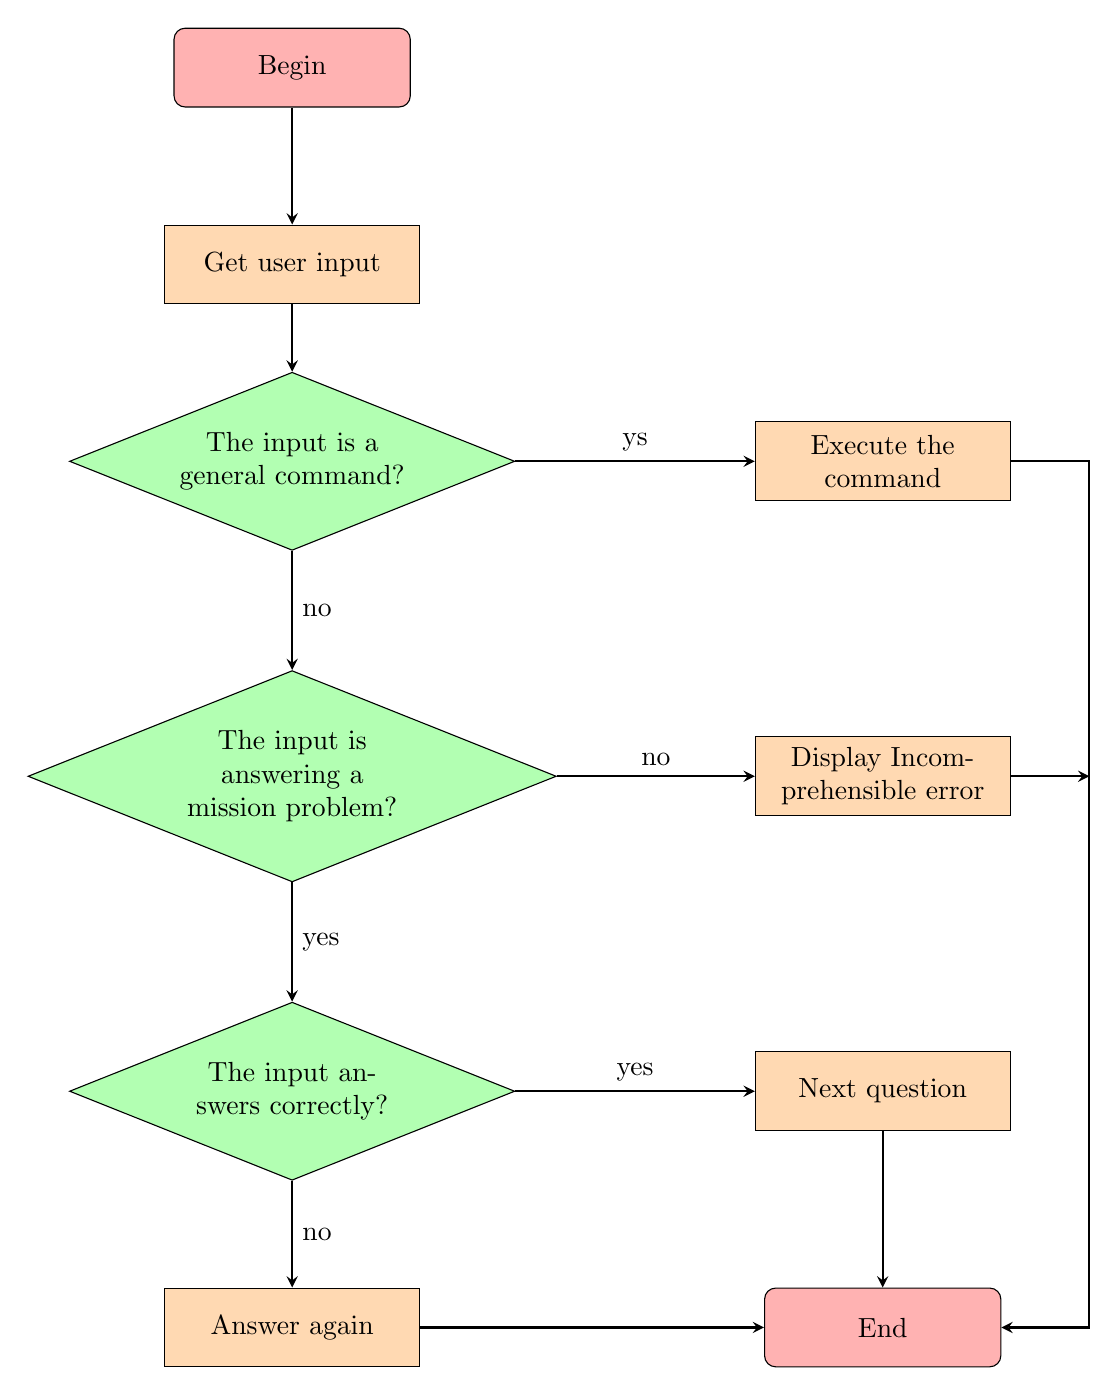
\begin{tikzpicture}[node distance=2.5cm]

\node(begin)[startstop]{Begin};
\node(input)[process, below of=begin]{Get user input};
\node(command)[decision, below of=input, aspect=2.5]{The input is a general
command?};
\node(comm)[process, right of=command, xshift=5cm, aspect=2.5]{Execute the
command};
\node(misAns)[decision, below of=command, aspect=2.5, yshift=-1.5cm]{The input
is answering a mission problem?};
\node(misError)[process, right of=misAns, xshift=5cm, text width=3cm]{Display
Incomprehensible error};
\node(ans)[decision, below of=misAns, aspect=2.5, yshift=-1.5cm]{The input
answers correctly?};
\node(next)[process, right of=ans, xshift=5cm]{Next question};
\node(again)[process, below of=ans, yshift=-0.5cm]{Answer again};
\node(end)[startstop, right of=again, xshift=5cm]{End};

\draw[arrow](begin) -- (input);
\draw[arrow](input) -- (command);
\draw[arrow](command) -- node[anchor=south]{ys}(comm);
\draw[arrow](command) -- node[anchor=west]{no}(misAns);
\draw[arrow](misAns) -- node[anchor=south]{no}(misError);
\draw[arrow](misAns) -- node[anchor=west]{yes}(ans);
\draw[arrow](ans) -- node[anchor=south]{yes}(next);
\draw[arrow](ans) -- node[anchor=west]{no}(again);
\draw[arrow](next) -- (end);
\draw[arrow](again) -- (end);
\draw[arrow](misError) -- ([xshift=1cm]misError.east);
\draw[arrow](comm) -- ([xshift=1cm]comm.east) |- (end);

\end{tikzpicture}
\subsubsection{Commands}
The following commands are planned as a general commands for the whole game
instead of a particular mission, those in bracket are shortcut:
\emph{save} (\emph{s}), \emph{quit} (\emph{q}),\emph{help} (\emph{h}),
\emph{load}, \emph{myinfo}, and \emph{feedback}.

\subsection{Game-ending Decision}
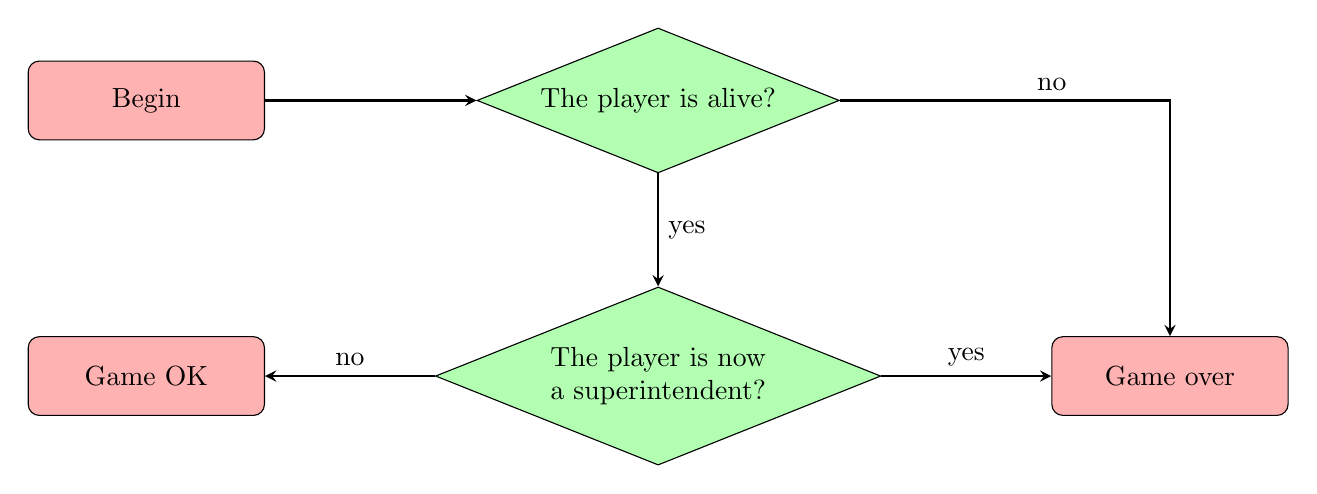
\begin{tikzpicture}[node distance=2.5cm]

\node(begin)[startstop]{Begin};
\node(alive)[decision, right of=begin, xshift=4cm, aspect=2.5]{The player is
alive?};
\node(rank)[decision, below of=alive, aspect=2.5, yshift=-1cm]{The player is now
a superintendent?};
\node(good)[startstop, below of=begin, yshift=-1cm]{Game OK};
\node(bad)[startstop, right of=rank, xshift=4cm]{Game over};

\draw[arrow](begin) -- (alive);
\draw[arrow](alive) node[anchor=south, xshift=5cm]{no} -| (bad);
\draw[arrow](alive) -- node[anchor=west]{yes}(rank);
\draw[arrow](rank) -- node[anchor=south]{no}(good);
\draw[arrow](rank) -- node[anchor=south]{yes}(bad);

\end{tikzpicture}

\clearpage
% UI example
\section{User Interface}
\begin{figure}[h]
\begin{subfigure}[b]{0.4\textwidth}
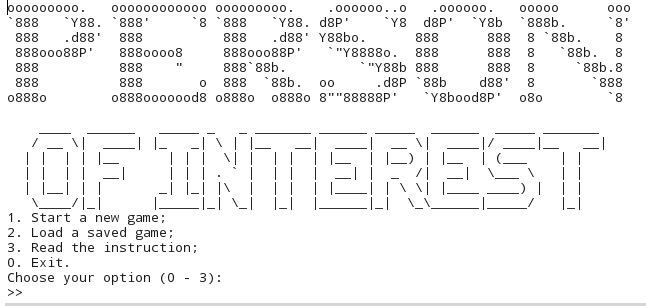
\includegraphics[width=\linewidth]{./img/ui1}
\caption{start page}
\end{subfigure}
~
\begin{subfigure}[b]{0.4\textwidth}
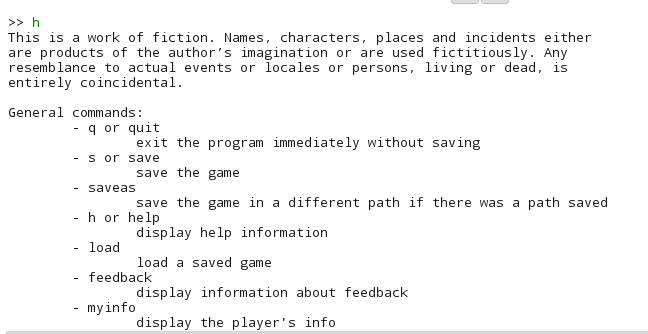
\includegraphics[width=\linewidth]{./img/ui2}
\caption{help document}
\end{subfigure}

\begin{subfigure}[b]{0.4\textwidth}
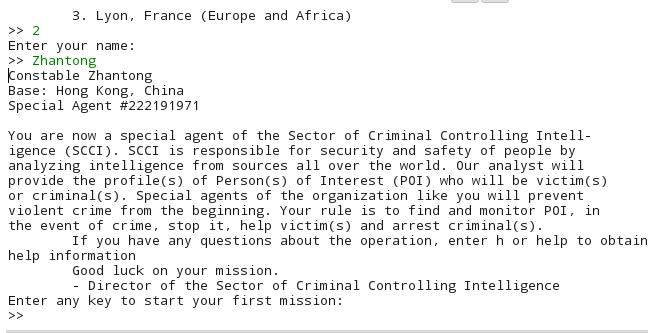
\includegraphics[width=\linewidth]{./img/ui3}
\caption{game beginning}
\end{subfigure}
~
\begin{subfigure}[b]{0.4\textwidth}
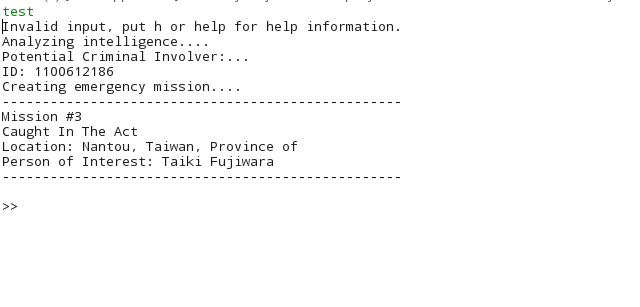
\includegraphics[width=\linewidth]{./img/ui4}
\caption{mission generation}
\end{subfigure}
\caption{UI examples}
\end{figure}

% source
\part{Program Source}
% list settings
\lstset{language=Java, numbers=left, breaklines=true, showstringspaces=false,
basicstyle=\footnotesize\ttfamily, tabsize=2,keywordstyle=\bfseries}
% source
\chapter{Source}
The source code of the program can be also found at
\url{https://github.com/zhantongz/person-of-interest} with other program
resources, and \LaTeX\ sources and generated PDFs of the program documents.

The Java source code and program resources are placed in different directory.
\texttt{src} is for program source that define how the program work. And
\texttt{res} is for resources that provide meaningful resources to be processed
by the program.

\section{Agent.java}
\lstinputlisting{../personOfInterest/src/personOfInterest/Agent.java}

\section{Game.java}
\lstinputlisting{../personOfInterest/src/personOfInterest/Game.java}

\section{Location.java}
\lstinputlisting{../personOfInterest/src/personOfInterest/Location.java}

\section{Mission.java}
\lstinputlisting{../personOfInterest/src/personOfInterest/Mission.java}

\section{Person.java}
\lstinputlisting{../personOfInterest/src/personOfInterest/Person.java}

\section{Player.java}
\lstinputlisting{../personOfInterest/src/personOfInterest/Player.java}

\section{POI.java}
\lstinputlisting{../personOfInterest/src/personOfInterest/POI.java}

\section{Problem.java}
\lstinputlisting{../personOfInterest/src/personOfInterest/Problem.java}

\section{Saved.java}
\lstinputlisting{../personOfInterest/src/personOfInterest/Saved.java}

Program resources are not included because of their large sizes and the inability to show source (like binary files). Those resources will be updated and can be obtained from the git repository at \url{https://github.com/zhantongz/person-of-interest}. The following are examples of text resources.
\section{locs.csv}
This file contains information of locations in the game.
\lstinputlisting{../personOfInterest/res/locs/locs.csv}

\section{mst/1.csv}
This file is description for the first mission.
\lstinputlisting{../personOfInterest/res/msts/1.csv}

\section{prbs/1.csv}
This file contains problems in the first mission.
\lstinputlisting{../personOfInterest/res/prbs/1.csv}
% evaluation
\part{Evaluation}
% general evaluation
Over all, this project contains 1056 lines of Java codes.
% program structure and document
\chapter{Program Structure}
The detailed description of classes, constants, methods and variables are listed in this chapter, following the alphabetical order of class names. The purpose and the parameter and return value for methods are described in order to provide a development guide for others. This chapter is automatically generated with \texttt{javadoc} using TeXDoclet at \url{http://doclet.github.io/} from the source code.
\sloppy
\section{\label{personOfInterest.Agent}\index{Agent}Class Agent}{
\vskip .1in 
Agent of the organization \\ref: \url{http://docs.oracle.com/javase/tutorial/java/javaOO/index.html}\vskip .1in 
\subsection{Declaration}{
\small public class Agent
\\ {\bf  extends} personOfInterest.Person
\refdefined{personOfInterest.Person}}
\subsection{All known subclasses}{Player\small{\refdefined{personOfInterest.Player}}}
\subsection{Field summary}{
\begin{verse}
{\bf base} base location of an agent\\
{\bf calendar} calendar of an agent\\
{\bf currentDay} current day in the calendar\\
{\bf id} an agent's id number\\
{\bf rank} rank of an agent\\
{\bf RANKS} ranks' list \\ref: \url{http://java.about.com/od/understandingdatatypes/a/Using-Constants.htm}\\
{\bf serialVersionUID} serialization id\\
\end{verse}
}
\subsection{Constructor summary}{
\begin{verse}
{\bf Agent(String, int, Location)} Construct a new agent with specified name, rank and base location and a random id\\
{\bf Agent(String, int, Location, int)} Construct a new agent with specified name, rank and base location and a random id\\
\end{verse}
}
\subsection{Method summary}{
\begin{verse}
{\bf displayInfo()} Display an agent's info including rank, name, base and ID\\
{\bf passDay()} Pass current day\\
{\bf passDays(int)} Pass a certain number of days\\
{\bf resetCal()} Reset calendar of an agent\\
{\bf resetCal(int)} Reset calendar of an agent to a certain period\\
\end{verse}
}
\subsection{Fields}{
\begin{itemize}
\item{
\index{serialVersionUID}
\label{personOfInterest.Agent.serialVersionUID}private static final long {\bf  serialVersionUID}\begin{itemize}
\item{\vskip -.9ex 
serialization id}
\end{itemize}
}
\item{
\index{base}
\label{personOfInterest.Agent.base} Location {\bf  base}\begin{itemize}
\item{\vskip -.9ex 
base location of an agent}
\end{itemize}
}
\item{
\index{id}
\label{personOfInterest.Agent.id} int {\bf  id}\begin{itemize}
\item{\vskip -.9ex 
an agent's id number}
\end{itemize}
}
\item{
\index{rank}
\label{personOfInterest.Agent.rank} int {\bf  rank}\begin{itemize}
\item{\vskip -.9ex 
rank of an agent}
\end{itemize}
}
\item{
\index{RANKS}
\label{personOfInterest.Agent.RANKS}public static final java.lang.String {\bf  RANKS}\begin{itemize}
\item{\vskip -.9ex 
ranks' list \\ref: \url{http://java.about.com/od/understandingdatatypes/a/Using-Constants.htm}}
\end{itemize}
}
\item{
\index{calendar}
\label{personOfInterest.Agent.calendar} int {\bf  calendar}\begin{itemize}
\item{\vskip -.9ex 
calendar of an agent}
\end{itemize}
}
\item{
\index{currentDay}
\label{personOfInterest.Agent.currentDay} int {\bf  currentDay}\begin{itemize}
\item{\vskip -.9ex 
current day in the calendar}
\end{itemize}
}
\end{itemize}
}
\subsection{Constructors}{
\vskip -2em
\begin{itemize}
\item{ 
\index{Agent(String, int, Location)}
{\bf  Agent}\\
\texttt{public\ {\bf  Agent}(\texttt{java.lang.String} {\bf  inName},
\texttt{int} {\bf  inRank},
\texttt{Location} {\bf  inBase})
\label{personOfInterest.Agent(java.lang.String, int, personOfInterest.Location)}}%end signature
\begin{itemize}
\item{
{\bf  Description}

Construct a new agent with specified name, rank and base location and a random id
}
\item{
{\bf  Parameters}
  \begin{itemize}
   \item{
\texttt{inName} -- specified name for the new agent}
   \item{
\texttt{inRank} -- specified rank for the new agent}
   \item{
\texttt{inBase} -- specified base location for the new agent}
  \end{itemize}
}%end item
\end{itemize}
}%end item
\item{ 
\index{Agent(String, int, Location, int)}
{\bf  Agent}\\
\texttt{public\ {\bf  Agent}(\texttt{java.lang.String} {\bf  inName},
\texttt{int} {\bf  inRank},
\texttt{Location} {\bf  inBase},
\texttt{int} {\bf  inId})
\label{personOfInterest.Agent(java.lang.String, int, personOfInterest.Location, int)}}%end signature
\begin{itemize}
\item{
{\bf  Description}

Construct a new agent with specified name, rank and base location and a random id
}
\item{
{\bf  Parameters}
  \begin{itemize}
   \item{
\texttt{inName} -- specified name for the new agent}
   \item{
\texttt{inRank} -- specified rank for the new agent}
   \item{
\texttt{inBase} -- specified base location for the new agent}
   \item{
\texttt{inId} -- specified id number for the new agent}
  \end{itemize}
}%end item
\end{itemize}
}%end item
\end{itemize}
}
\subsection{Methods}{
\vskip -2em
\begin{itemize}
\item{ 
\index{displayInfo()}
{\bf  displayInfo}\\
\texttt{public void\ {\bf  displayInfo}()
\label{personOfInterest.Agent.displayInfo()}}%end signature
\begin{itemize}
\item{
{\bf  Description}

Display an agent's info including rank, name, base and ID
}
\end{itemize}
}%end item
\item{ 
\index{passDay()}
{\bf  passDay}\\
\texttt{public void\ {\bf  passDay}()
\label{personOfInterest.Agent.passDay()}}%end signature
\begin{itemize}
\item{
{\bf  Description}

Pass current day
}
\end{itemize}
}%end item
\item{ 
\index{passDays(int)}
{\bf  passDays}\\
\texttt{public void\ {\bf  passDays}(\texttt{int} {\bf  days})
\label{personOfInterest.Agent.passDays(int)}}%end signature
\begin{itemize}
\item{
{\bf  Description}

Pass a certain number of days
}
\item{
{\bf  Parameters}
  \begin{itemize}
   \item{
\texttt{days} -- the number of days passed}
  \end{itemize}
}%end item
\end{itemize}
}%end item
\item{ 
\index{resetCal()}
{\bf  resetCal}\\
\texttt{public void\ {\bf  resetCal}()
\label{personOfInterest.Agent.resetCal()}}%end signature
\begin{itemize}
\item{
{\bf  Description}

Reset calendar of an agent
}
\end{itemize}
}%end item
\item{ 
\index{resetCal(int)}
{\bf  resetCal}\\
\texttt{public void\ {\bf  resetCal}(\texttt{int} {\bf  days})
\label{personOfInterest.Agent.resetCal(int)}}%end signature
\begin{itemize}
\item{
{\bf  Description}

Reset calendar of an agent to a certain period
}
\end{itemize}
}%end item
\end{itemize}
}
\subsection{Members inherited from class Person }{
\texttt{personOfInterest.Person} {\small 
\refdefined{personOfInterest.Person}}
{\small 

\vskip -2em
\begin{itemize}
\item{\vskip -1.5ex 
\texttt{public void {\bf  displayInfo}()
}%end signature
}%end item
\item{\vskip -1.5ex 
\texttt{ {\bf  ifAlive}}%end signature
}%end item
\item{\vskip -1.5ex 
\texttt{public void {\bf  kill}()
}%end signature
}%end item
\item{\vskip -1.5ex 
\texttt{ {\bf  location}}%end signature
}%end item
\item{\vskip -1.5ex 
\texttt{ {\bf  name}}%end signature
}%end item
\item{\vskip -1.5ex 
\texttt{private static final {\bf  serialVersionUID}}%end signature
}%end item
\end{itemize}
}
}
\section{\label{personOfInterest.Game}\index{Game}Class Game}{
\vskip .1in 
Main game program\vskip .1in 
\subsection{Declaration}{
\small public class Game
\\ {\bf  extends} java.lang.Object
\refdefined{java.lang.Object}}
\subsection{Field summary}{
\begin{verse}
{\bf gameCal} game calendar\\
{\bf input} scanner that reads from keyboard\\
{\bf locArea} \\
{\bf newMission} if the player wants to start a new mission\\
{\bf poiArea} \\
{\bf processed} \\
{\bf savedName} saved name for saving game\\
{\bf savedPath} saved path for saving game\\
\end{verse}
}
\subsection{Method summary}{
\begin{verse}
{\bf addLinebreaks(String)} Break lines in a long string with maximum length of 80\\
{\bf addLinebreaks(String, int)} Break lines in a long string to make display nicer \\ref: \url{http://stackoverflow.com/questions/7528045/large-string-split-into- lines-with-maximum-length-in-java}\\
{\bf displayDate()} Display the date today (as in the game)\\
{\bf help()} Display help information\\
{\bf ifGoodCalendar(int\lbrack \rbrack )} Determine if a player complete his/her mission in a certain time\\
{\bf input(String)} Get the user's input with space as the delimiter\\
{\bf input(String, int, int)} Check if the user's input is valid and return a valid data\\
{\bf inputLn(String)} Get the user's input with line break as the delimiter\\
{\bf isGameOver(Player)} Determine if the game is over\\
{\bf loadFile(String)} Load a serialized file\\
{\bf locs()} Update location information from the csv file\\
{\bf main(String\lbrack \rbrack )} Main program\\
{\bf msts()} Update location information from the csv file\\
{\bf passDay()} Add 1 day to the calendar\\
{\bf passDays(int)} Add a certain number of days to the game calendar\\
{\bf pois()} Update location information from the csv file\\
{\bf prbs()} Update problems\\
{\bf processUserInput(Problem, Player)} Process the user's input that intends for a problem\\
{\bf processUserInput(String, Player)} Process the user's input\\
{\bf randomID()} Generate a 9-digits id number for agent id, mission id, etc.\\
{\bf randomNum(int, int)} Generate a random number in a certain range\\
{\bf saveGame(Player)} Save the game\\
{\bf scciSeal()} Print SCCI logo\\
{\bf showStartPage()} Show the start page with ASCII art\\
{\bf sleep(int)} Pause the program for a period of time while outputing three dots \\ref: \url{http://docs.oracle.com/javase/tutorial/essential/concurrency/sleep.html}\\
{\bf takeChance(double)} \\
{\bf takeChance(int)} \\
{\bf toBoolean(int)} Cast int to boolean\\
{\bf transport(Agent, int, Location, Location)} Transport an agent from his/her current location to a location requested through a certain way\\
{\bf typeString(String)} Show a string in typewriter style\\
\end{verse}
}
\subsection{Fields}{
\begin{itemize}
\item{
\index{input}
\label{personOfInterest.Game.input}static java.util.Scanner {\bf  input}\begin{itemize}
\item{\vskip -.9ex 
scanner that reads from keyboard}
\end{itemize}
}
\item{
\index{savedPath}
\label{personOfInterest.Game.savedPath}static java.lang.String {\bf  savedPath}\begin{itemize}
\item{\vskip -.9ex 
saved path for saving game}
\end{itemize}
}
\item{
\index{savedName}
\label{personOfInterest.Game.savedName}static java.lang.String {\bf  savedName}\begin{itemize}
\item{\vskip -.9ex 
saved name for saving game}
\end{itemize}
}
\item{
\index{gameCal}
\label{personOfInterest.Game.gameCal}static java.util.Calendar {\bf  gameCal}\begin{itemize}
\item{\vskip -.9ex 
game calendar}
\end{itemize}
}
\item{
\index{locArea}
\label{personOfInterest.Game.locArea}static int {\bf  locArea}}
\item{
\index{poiArea}
\label{personOfInterest.Game.poiArea}static int {\bf  poiArea}}
\item{
\index{newMission}
\label{personOfInterest.Game.newMission}static boolean {\bf  newMission}\begin{itemize}
\item{\vskip -.9ex 
if the player wants to start a new mission}
\end{itemize}
}
\item{
\index{processed}
\label{personOfInterest.Game.processed}static boolean {\bf  processed}}
\end{itemize}
}
\subsection{Methods}{
\vskip -2em
\begin{itemize}
\item{ 
\index{addLinebreaks(String)}
{\bf  addLinebreaks}\\
\texttt{public static java.lang.String\ {\bf  addLinebreaks}(\texttt{java.lang.String} {\bf  input})
\label{personOfInterest.Game.addLinebreaks(java.lang.String)}}%end signature
\begin{itemize}
\item{
{\bf  Description}

Break lines in a long string with maximum length of 80
}
\item{
{\bf  Parameters}
  \begin{itemize}
   \item{
\texttt{input} -- the string need to be broken}
  \end{itemize}
}%end item
\item{{\bf  Returns} -- 
the string with proper breaks 
}%end item
\end{itemize}
}%end item
\item{ 
\index{addLinebreaks(String, int)}
{\bf  addLinebreaks}\\
\texttt{public static java.lang.String\ {\bf  addLinebreaks}(\texttt{java.lang.String} {\bf  input},
\texttt{int} {\bf  maxLineLength})
\label{personOfInterest.Game.addLinebreaks(java.lang.String, int)}}%end signature
\begin{itemize}
\item{
{\bf  Description}

Break lines in a long string to make display nicer \\ref: \url{http://stackoverflow.com/questions/7528045/large-string-split-into- lines-with-maximum-length-in-java}
}
\item{
{\bf  Parameters}
  \begin{itemize}
   \item{
\texttt{input} -- the string need to be broken}
   \item{
\texttt{maxLineLength} -- the maxium line length to insert break line}
  \end{itemize}
}%end item
\item{{\bf  Returns} -- 
the string with proper breaks 
}%end item
\end{itemize}
}%end item
\item{ 
\index{displayDate()}
{\bf  displayDate}\\
\texttt{public static java.lang.String\ {\bf  displayDate}()
\label{personOfInterest.Game.displayDate()}}%end signature
\begin{itemize}
\item{
{\bf  Description}

Display the date today (as in the game)
}
\item{{\bf  Returns} -- 
the current date in the game 
}%end item
\end{itemize}
}%end item
\item{ 
\index{help()}
{\bf  help}\\
\texttt{public static void\ {\bf  help}() throws java.io.FileNotFoundException
\label{personOfInterest.Game.help()}}%end signature
\begin{itemize}
\item{
{\bf  Description}

Display help information
}
\end{itemize}
}%end item
\item{ 
\index{ifGoodCalendar(int\lbrack \rbrack )}
{\bf  ifGoodCalendar}\\
\texttt{public static boolean\ {\bf  ifGoodCalendar}(\texttt{int\lbrack \rbrack } {\bf  calendar})
\label{personOfInterest.Game.ifGoodCalendar(int[])}}%end signature
\begin{itemize}
\item{
{\bf  Description}

Determine if a player complete his/her mission in a certain time
}
\item{
{\bf  Parameters}
  \begin{itemize}
   \item{
\texttt{calendar} -- the calendar of the player/mission}
  \end{itemize}
}%end item
\item{{\bf  Returns} -- 
true if the player doesn't fail to comply the calendar; false otherwise 
}%end item
\end{itemize}
}%end item
\item{ 
\index{input(String)}
{\bf  input}\\
\texttt{public static java.lang.String\ {\bf  input}(\texttt{java.lang.String} {\bf  prompt}) throws java.io.IOException
\label{personOfInterest.Game.input(java.lang.String)}}%end signature
\begin{itemize}
\item{
{\bf  Description}

Get the user's input with space as the delimiter
}
\item{
{\bf  Parameters}
  \begin{itemize}
   \item{
\texttt{prompt} -- prompt for the user}
  \end{itemize}
}%end item
\item{{\bf  Returns} -- 
the string user entered 
}%end item
\end{itemize}
}%end item
\item{ 
\index{input(String, int, int)}
{\bf  input}\\
\texttt{public static int\ {\bf  input}(\texttt{java.lang.String} {\bf  prompt},
\texttt{int} {\bf  min},
\texttt{int} {\bf  max})
\label{personOfInterest.Game.input(java.lang.String, int, int)}}%end signature
\begin{itemize}
\item{
{\bf  Description}

Check if the user's input is valid and return a valid data
}
\item{
{\bf  Parameters}
  \begin{itemize}
   \item{
\texttt{prompt} -- prompt for the user}
   \item{
\texttt{min} -- the minimum value for a valid data}
   \item{
\texttt{max} -- the maximum value for a valid data}
  \end{itemize}
}%end item
\item{{\bf  Returns} -- 
a valid integer data between min and max 
}%end item
\end{itemize}
}%end item
\item{ 
\index{inputLn(String)}
{\bf  inputLn}\\
\texttt{public static java.lang.String\ {\bf  inputLn}(\texttt{java.lang.String} {\bf  prompt})
\label{personOfInterest.Game.inputLn(java.lang.String)}}%end signature
\begin{itemize}
\item{
{\bf  Description}

Get the user's input with line break as the delimiter
}
\item{
{\bf  Parameters}
  \begin{itemize}
   \item{
\texttt{prompt} -- prompt for the user}
  \end{itemize}
}%end item
\item{{\bf  Returns} -- 
the string user entered 
}%end item
\end{itemize}
}%end item
\item{ 
\index{isGameOver(Player)}
{\bf  isGameOver}\\
\texttt{public static boolean\ {\bf  isGameOver}(\texttt{Player} {\bf  player})
\label{personOfInterest.Game.isGameOver(personOfInterest.Player)}}%end signature
\begin{itemize}
\item{
{\bf  Description}

Determine if the game is over
}
\item{{\bf  Returns} -- 
true if the player is alive and not completed the game; false otherwise 
}%end item
\end{itemize}
}%end item
\item{ 
\index{loadFile(String)}
{\bf  loadFile}\\
\texttt{public static java.lang.Object\ {\bf  loadFile}(\texttt{java.lang.String} {\bf  prompt}) throws java.io.IOException
\label{personOfInterest.Game.loadFile(java.lang.String)}}%end signature
\begin{itemize}
\item{
{\bf  Description}

Load a serialized file
}
\item{
{\bf  Parameters}
  \begin{itemize}
   \item{
\texttt{prompt} -- prompt for the user}
  \end{itemize}
}%end item
\item{{\bf  Returns} -- 
the object included in the file 
}%end item
\end{itemize}
}%end item
\item{ 
\index{locs()}
{\bf  locs}\\
\texttt{public static void\ {\bf  locs}() throws java.lang.NumberFormatException, java.io.IOException, java.lang.InterruptedException
\label{personOfInterest.Game.locs()}}%end signature
\begin{itemize}
\item{
{\bf  Description}

Update location information from the csv file
}
\end{itemize}
}%end item
\item{ 
\index{main(String\lbrack \rbrack )}
{\bf  main}\\
\texttt{public static void\ {\bf  main}(\texttt{java.lang.String\lbrack \rbrack } {\bf  args}) throws java.io.IOException, java.lang.ClassNotFoundException, java.lang.InterruptedException
\label{personOfInterest.Game.main(java.lang.String[])}}%end signature
\begin{itemize}
\item{
{\bf  Description}

Main program
}
\end{itemize}
}%end item
\item{ 
\index{msts()}
{\bf  msts}\\
\texttt{public static void\ {\bf  msts}() throws java.lang.NumberFormatException, java.io.IOException, java.lang.InterruptedException
\label{personOfInterest.Game.msts()}}%end signature
\begin{itemize}
\item{
{\bf  Description}

Update location information from the csv file
}
\end{itemize}
}%end item
\item{ 
\index{passDay()}
{\bf  passDay}\\
\texttt{public static void\ {\bf  passDay}()
\label{personOfInterest.Game.passDay()}}%end signature
\begin{itemize}
\item{
{\bf  Description}

Add 1 day to the calendar
}
\end{itemize}
}%end item
\item{ 
\index{passDays(int)}
{\bf  passDays}\\
\texttt{public static void\ {\bf  passDays}(\texttt{int} {\bf  days})
\label{personOfInterest.Game.passDays(int)}}%end signature
\begin{itemize}
\item{
{\bf  Description}

Add a certain number of days to the game calendar
}
\item{
{\bf  Parameters}
  \begin{itemize}
   \item{
\texttt{days} -- the certain number of days}
  \end{itemize}
}%end item
\end{itemize}
}%end item
\item{ 
\index{pois()}
{\bf  pois}\\
\texttt{public static void\ {\bf  pois}() throws java.lang.NumberFormatException, java.io.IOException, java.lang.InterruptedException
\label{personOfInterest.Game.pois()}}%end signature
\begin{itemize}
\item{
{\bf  Description}

Update location information from the csv file
}
\end{itemize}
}%end item
\item{ 
\index{prbs()}
{\bf  prbs}\\
\texttt{public static void\ {\bf  prbs}() throws java.io.IOException
\label{personOfInterest.Game.prbs()}}%end signature
\begin{itemize}
\item{
{\bf  Description}

Update problems
}
\end{itemize}
}%end item
\item{ 
\index{processUserInput(Problem, Player)}
{\bf  processUserInput}\\
\texttt{public static boolean\ {\bf  processUserInput}(\texttt{Problem} {\bf  problem},
\texttt{Player} {\bf  player}) throws java.io.IOException, java.lang.ClassNotFoundException, java.lang.InterruptedException
\label{personOfInterest.Game.processUserInput(personOfInterest.Problem, personOfInterest.Player)}}%end signature
\begin{itemize}
\item{
{\bf  Description}

Process the user's input that intends for a problem
}
\item{
{\bf  Parameters}
  \begin{itemize}
   \item{
\texttt{problem} -- the problem}
   \item{
\texttt{player} -- the player}
  \end{itemize}
}%end item
\item{{\bf  Returns} -- 
true if the user answers the question correctly; false if answers incorrectly or doesn't answer 
}%end item
\end{itemize}
}%end item
\item{ 
\index{processUserInput(String, Player)}
{\bf  processUserInput}\\
\texttt{public static boolean\ {\bf  processUserInput}(\texttt{java.lang.String} {\bf  uInput},
\texttt{Player} {\bf  player}) throws java.io.FileNotFoundException, java.io.IOException, java.lang.ClassNotFoundException, java.lang.InterruptedException
\label{personOfInterest.Game.processUserInput(java.lang.String, personOfInterest.Player)}}%end signature
\begin{itemize}
\item{
{\bf  Description}

Process the user's input
}
\item{
{\bf  Parameters}
  \begin{itemize}
   \item{
\texttt{uinput} -- the user's input}
   \item{
\texttt{player} -- the player}
  \end{itemize}
}%end item
\item{{\bf  Returns} -- 
true if the input is processed; false otherwise 
}%end item
\end{itemize}
}%end item
\item{ 
\index{randomID()}
{\bf  randomID}\\
\texttt{public static int\ {\bf  randomID}()
\label{personOfInterest.Game.randomID()}}%end signature
\begin{itemize}
\item{
{\bf  Description}

Generate a 9-digits id number for agent id, mission id, etc.
}
\item{{\bf  Returns} -- 
the generated 9-digits number 
}%end item
\end{itemize}
}%end item
\item{ 
\index{randomNum(int, int)}
{\bf  randomNum}\\
\texttt{public static int\ {\bf  randomNum}(\texttt{int} {\bf  min},
\texttt{int} {\bf  max})
\label{personOfInterest.Game.randomNum(int, int)}}%end signature
\begin{itemize}
\item{
{\bf  Description}

Generate a random number in a certain range
}
\item{
{\bf  Parameters}
  \begin{itemize}
   \item{
\texttt{min} -- the minimum for the number, inclusive}
   \item{
\texttt{max} -- the maximum for the number, inclusive}
  \end{itemize}
}%end item
\item{{\bf  Returns} -- 
the generated number 
}%end item
\end{itemize}
}%end item
\item{ 
\index{saveGame(Player)}
{\bf  saveGame}\\
\texttt{public static boolean\ {\bf  saveGame}(\texttt{Player} {\bf  player}) throws java.io.FileNotFoundException, java.io.IOException
\label{personOfInterest.Game.saveGame(personOfInterest.Player)}}%end signature
\begin{itemize}
\item{
{\bf  Description}

Save the game
}
\item{
{\bf  Parameters}
  \begin{itemize}
   \item{
\texttt{player} -- the game's player}
  \end{itemize}
}%end item
\item{{\bf  Returns} -- 
true if the saving is a success; false otherwise 
}%end item
\end{itemize}
}%end item
\item{ 
\index{scciSeal()}
{\bf  scciSeal}\\
\texttt{public static void\ {\bf  scciSeal}()
\label{personOfInterest.Game.scciSeal()}}%end signature
\begin{itemize}
\item{
{\bf  Description}

Print SCCI logo
}
\end{itemize}
}%end item
\item{ 
\index{showStartPage()}
{\bf  showStartPage}\\
\texttt{public static void\ {\bf  showStartPage}()
\label{personOfInterest.Game.showStartPage()}}%end signature
\begin{itemize}
\item{
{\bf  Description}

Show the start page with ASCII art
}
\end{itemize}
}%end item
\item{ 
\index{sleep(int)}
{\bf  sleep}\\
\texttt{public static void\ {\bf  sleep}(\texttt{int} {\bf  timeInMs}) throws java.lang.InterruptedException
\label{personOfInterest.Game.sleep(int)}}%end signature
\begin{itemize}
\item{
{\bf  Description}

Pause the program for a period of time while outputing three dots \\ref: \url{http://docs.oracle.com/javase/tutorial/essential/concurrency/sleep.html}
}
\item{
{\bf  Parameters}
  \begin{itemize}
   \item{
\texttt{timeInMs} -- the period of time to be paused for}
  \end{itemize}
}%end item
\end{itemize}
}%end item
\item{ 
\index{takeChance(double)}
{\bf  takeChance}\\
\texttt{public static boolean\ {\bf  takeChance}(\texttt{double} {\bf  chance})
\label{personOfInterest.Game.takeChance(double)}}%end signature
}%end item
\item{ 
\index{takeChance(int)}
{\bf  takeChance}\\
\texttt{public static boolean\ {\bf  takeChance}(\texttt{int} {\bf  divisor})
\label{personOfInterest.Game.takeChance(int)}}%end signature
}%end item
\item{ 
\index{toBoolean(int)}
{\bf  toBoolean}\\
\texttt{public static boolean\ {\bf  toBoolean}(\texttt{int} {\bf  num})
\label{personOfInterest.Game.toBoolean(int)}}%end signature
\begin{itemize}
\item{
{\bf  Description}

Cast int to boolean
}
\item{
{\bf  Parameters}
  \begin{itemize}
   \item{
\texttt{num} -- the int ready to be casted}
  \end{itemize}
}%end item
\item{{\bf  Returns} -- 
false if the int is 0; true otherwise 
}%end item
\end{itemize}
}%end item
\item{ 
\index{transport(Agent, int, Location, Location)}
{\bf  transport}\\
\texttt{public static void\ {\bf  transport}(\texttt{Agent} {\bf  agent},
\texttt{int} {\bf  method},
\texttt{Location} {\bf  from},
\texttt{Location} {\bf  to})
\label{personOfInterest.Game.transport(personOfInterest.Agent, int, personOfInterest.Location, personOfInterest.Location)}}%end signature
\begin{itemize}
\item{
{\bf  Description}

Transport an agent from his/her current location to a location requested through a certain way
}
\item{
{\bf  Parameters}
  \begin{itemize}
   \item{
\texttt{agent} -- the agent that need to be transported}
   \item{
\texttt{method} -- the way of transportation; 1 for train, 2 for plane, 3 for normal vehicle and 4 for high-speed rail}
   \item{
\texttt{from} -- the current location}
   \item{
\texttt{to} -- the location requested}
  \end{itemize}
}%end item
\end{itemize}
}%end item
\item{ 
\index{typeString(String)}
{\bf  typeString}\\
\texttt{public static void\ {\bf  typeString}(\texttt{java.lang.String} {\bf  message}) throws java.lang.InterruptedException
\label{personOfInterest.Game.typeString(java.lang.String)}}%end signature
\begin{itemize}
\item{
{\bf  Description}

Show a string in typewriter style
}
\item{
{\bf  Parameters}
  \begin{itemize}
   \item{
\texttt{message} -- the string need to be displayed}
  \end{itemize}
}%end item
\end{itemize}
}%end item
\end{itemize}
}
}
\section{\label{personOfInterest.Location}\index{Location}Class Location}{
\vskip .1in 
Location\vskip .1in 
\subsection{Declaration}{
\small public class Location
\\ {\bf  extends} java.lang.Object
\refdefined{java.lang.Object}\\ {\bf  implements} 
java.io.Serializable}
\subsection{Field summary}{
\begin{verse}
{\bf area} a location's area as the index in AREAS\\
{\bf AREAS} areas that a location can be included in\\
{\bf city} city that a location situated\\
{\bf country} country that a location situated\\
{\bf description} description of a location\\
{\bf name} a location's name\\
{\bf serialVersionUID} serialization id\\
{\bf sublocations} locations that are in a location\\
{\bf subNum} the number of sublocations\\
\end{verse}
}
\subsection{Constructor summary}{
\begin{verse}
{\bf Location(String, String, String, int, String)} Construct a location with name.\\
\end{verse}
}
\subsection{Method summary}{
\begin{verse}
{\bf addSublocation(Location)} Add a sublocation\\
{\bf addSublocations(Location\lbrack \rbrack )} Add a series of sublocation\\
\end{verse}
}
\subsection{Fields}{
\begin{itemize}
\item{
\index{serialVersionUID}
\label{personOfInterest.Location.serialVersionUID}private static final long {\bf  serialVersionUID}\begin{itemize}
\item{\vskip -.9ex 
serialization id}
\end{itemize}
}
\item{
\index{name}
\label{personOfInterest.Location.name} java.lang.String {\bf  name}\begin{itemize}
\item{\vskip -.9ex 
a location's name}
\end{itemize}
}
\item{
\index{area}
\label{personOfInterest.Location.area} int {\bf  area}\begin{itemize}
\item{\vskip -.9ex 
a location's area as the index in AREAS}
\end{itemize}
}
\item{
\index{city}
\label{personOfInterest.Location.city} java.lang.String {\bf  city}\begin{itemize}
\item{\vskip -.9ex 
city that a location situated}
\end{itemize}
}
\item{
\index{country}
\label{personOfInterest.Location.country} java.lang.String {\bf  country}\begin{itemize}
\item{\vskip -.9ex 
country that a location situated}
\end{itemize}
}
\item{
\index{sublocations}
\label{personOfInterest.Location.sublocations} Location {\bf  sublocations}\begin{itemize}
\item{\vskip -.9ex 
locations that are in a location}
\end{itemize}
}
\item{
\index{subNum}
\label{personOfInterest.Location.subNum} int {\bf  subNum}\begin{itemize}
\item{\vskip -.9ex 
the number of sublocations}
\end{itemize}
}
\item{
\index{description}
\label{personOfInterest.Location.description} java.lang.String {\bf  description}\begin{itemize}
\item{\vskip -.9ex 
description of a location}
\end{itemize}
}
\item{
\index{AREAS}
\label{personOfInterest.Location.AREAS}static final java.lang.String {\bf  AREAS}\begin{itemize}
\item{\vskip -.9ex 
areas that a location can be included in}
\end{itemize}
}
\end{itemize}
}
\subsection{Constructors}{
\vskip -2em
\begin{itemize}
\item{ 
\index{Location(String, String, String, int, String)}
{\bf  Location}\\
\texttt{public\ {\bf  Location}(\texttt{java.lang.String} {\bf  inName},
\texttt{java.lang.String} {\bf  inCity},
\texttt{java.lang.String} {\bf  inCountry},
\texttt{int} {\bf  inArea},
\texttt{java.lang.String} {\bf  inDescription})
\label{personOfInterest.Location(java.lang.String, java.lang.String, java.lang.String, int, java.lang.String)}}%end signature
\begin{itemize}
\item{
{\bf  Description}

Construct a location with name.
}
\item{
{\bf  Parameters}
  \begin{itemize}
   \item{
\texttt{inName} -- the location's name}
  \end{itemize}
}%end item
\end{itemize}
}%end item
\end{itemize}
}
\subsection{Methods}{
\vskip -2em
\begin{itemize}
\item{ 
\index{addSublocation(Location)}
{\bf  addSublocation}\\
\texttt{public void\ {\bf  addSublocation}(\texttt{Location} {\bf  subloc})
\label{personOfInterest.Location.addSublocation(personOfInterest.Location)}}%end signature
\begin{itemize}
\item{
{\bf  Description}

Add a sublocation
}
\item{
{\bf  Parameters}
  \begin{itemize}
   \item{
\texttt{subloc} -- the sublocation that needs to be added}
  \end{itemize}
}%end item
\end{itemize}
}%end item
\item{ 
\index{addSublocations(Location\lbrack \rbrack )}
{\bf  addSublocations}\\
\texttt{public void\ {\bf  addSublocations}(\texttt{Location\lbrack \rbrack } {\bf  sublocs})
\label{personOfInterest.Location.addSublocations(personOfInterest.Location[])}}%end signature
\begin{itemize}
\item{
{\bf  Description}

Add a series of sublocation
}
\item{
{\bf  Parameters}
  \begin{itemize}
   \item{
\texttt{sublocs} -- the sublocations that needs to be added}
  \end{itemize}
}%end item
\end{itemize}
}%end item
\end{itemize}
}
}
\section{\label{personOfInterest.Mission}\index{Mission}Class Mission}{
\vskip .1in 
Mission of the player\vskip .1in 
\subsection{Declaration}{
\small public class Mission
\\ {\bf  extends} java.lang.Object
\refdefined{java.lang.Object}}
\subsection{Field summary}{
\begin{verse}
{\bf arriveMessage} message displayed after arrival\\
{\bf budget} money that can be used to complete a mission\\
{\bf calendar} calendar of a mission; time permitted\\
{\bf completed} if a mission is completed\\
{\bf dangers} potential dangers of a mission\\
{\bf description} description of a mission\\
{\bf location} location that a mission takes place\\
{\bf minorNum} indication of where minor situations happens\\
{\bf name} name of a mission\\
{\bf player} player who is completing a mission\\
{\bf poi} person of interest in a mission\\
{\bf points} points that awarded after completion\\
{\bf prbNum} default number for problem\\
{\bf problems} situations in a mission\\
{\bf rank} rank that have abilities to complete a mission\\
\end{verse}
}
\subsection{Constructor summary}{
\begin{verse}
{\bf Mission(POI, String, Location, int, int)} Construct a mission\\
{\bf Mission(POI, String, Location, int, int, int)} \\
\end{verse}
}
\subsection{Method summary}{
\begin{verse}
{\bf complete()} Complete a mission\\
{\bf completing(int)} Process a mission\\
{\bf generateFinalMission(int)} Generate a final Mission\\
{\bf generateMission(int, int)} Generate a random mission\\
{\bf minorSituation(int, int)} Execute a customized minor situation\\
{\bf replaceName(String, Mission)} Replace certain tags in a string with certain variables\\
\end{verse}
}
\subsection{Fields}{
\begin{itemize}
\item{
\index{location}
\label{personOfInterest.Mission.location} Location {\bf  location}\begin{itemize}
\item{\vskip -.9ex 
location that a mission takes place}
\end{itemize}
}
\item{
\index{name}
\label{personOfInterest.Mission.name} java.lang.String {\bf  name}\begin{itemize}
\item{\vskip -.9ex 
name of a mission}
\end{itemize}
}
\item{
\index{poi}
\label{personOfInterest.Mission.poi} POI {\bf  poi}\begin{itemize}
\item{\vskip -.9ex 
person of interest in a mission}
\end{itemize}
}
\item{
\index{completed}
\label{personOfInterest.Mission.completed} boolean {\bf  completed}\begin{itemize}
\item{\vskip -.9ex 
if a mission is completed}
\end{itemize}
}
\item{
\index{rank}
\label{personOfInterest.Mission.rank} int {\bf  rank}\begin{itemize}
\item{\vskip -.9ex 
rank that have abilities to complete a mission}
\end{itemize}
}
\item{
\index{budget}
\label{personOfInterest.Mission.budget} int {\bf  budget}\begin{itemize}
\item{\vskip -.9ex 
money that can be used to complete a mission}
\end{itemize}
}
\item{
\index{calendar}
\label{personOfInterest.Mission.calendar} int {\bf  calendar}\begin{itemize}
\item{\vskip -.9ex 
calendar of a mission; time permitted}
\end{itemize}
}
\item{
\index{points}
\label{personOfInterest.Mission.points} int {\bf  points}\begin{itemize}
\item{\vskip -.9ex 
points that awarded after completion}
\end{itemize}
}
\item{
\index{player}
\label{personOfInterest.Mission.player} Player {\bf  player}\begin{itemize}
\item{\vskip -.9ex 
player who is completing a mission}
\end{itemize}
}
\item{
\index{dangers}
\label{personOfInterest.Mission.dangers} java.lang.String {\bf  dangers}\begin{itemize}
\item{\vskip -.9ex 
potential dangers of a mission}
\end{itemize}
}
\item{
\index{description}
\label{personOfInterest.Mission.description} java.lang.String {\bf  description}\begin{itemize}
\item{\vskip -.9ex 
description of a mission}
\end{itemize}
}
\item{
\index{problems}
\label{personOfInterest.Mission.problems} Problem {\bf  problems}\begin{itemize}
\item{\vskip -.9ex 
situations in a mission}
\end{itemize}
}
\item{
\index{arriveMessage}
\label{personOfInterest.Mission.arriveMessage} java.lang.String {\bf  arriveMessage}\begin{itemize}
\item{\vskip -.9ex 
message displayed after arrival}
\end{itemize}
}
\item{
\index{minorNum}
\label{personOfInterest.Mission.minorNum} int {\bf  minorNum}\begin{itemize}
\item{\vskip -.9ex 
indication of where minor situations happens}
\end{itemize}
}
\item{
\index{prbNum}
\label{personOfInterest.Mission.prbNum}static int {\bf  prbNum}\begin{itemize}
\item{\vskip -.9ex 
default number for problem}
\end{itemize}
}
\end{itemize}
}
\subsection{Constructors}{
\vskip -2em
\begin{itemize}
\item{ 
\index{Mission(POI, String, Location, int, int)}
{\bf  Mission}\\
\texttt{public\ {\bf  Mission}(\texttt{POI} {\bf  person},
\texttt{java.lang.String} {\bf  inname},
\texttt{Location} {\bf  inloc},
\texttt{int} {\bf  days},
\texttt{int} {\bf  inPoints})
\label{personOfInterest.Mission(personOfInterest.POI, java.lang.String, personOfInterest.Location, int, int)}}%end signature
\begin{itemize}
\item{
{\bf  Description}

Construct a mission
}
\item{
{\bf  Parameters}
  \begin{itemize}
   \item{
\texttt{person} -- the POI in a mission}
   \item{
\texttt{inname} -- the name of a mission}
   \item{
\texttt{inloc} -- the location of a mission}
   \item{
\texttt{days} -- the time limit in days for the mission}
   \item{
\texttt{inPoints} -- the points required to complete the mission}
  \end{itemize}
}%end item
\end{itemize}
}%end item
\item{ 
\index{Mission(POI, String, Location, int, int, int)}
{\bf  Mission}\\
\texttt{public\ {\bf  Mission}(\texttt{POI} {\bf  person},
\texttt{java.lang.String} {\bf  inname},
\texttt{Location} {\bf  inloc},
\texttt{int} {\bf  days},
\texttt{int} {\bf  inPoints},
\texttt{int} {\bf  rank}) throws java.io.FileNotFoundException, java.io.IOException, java.lang.ClassNotFoundException
\label{personOfInterest.Mission(personOfInterest.POI, java.lang.String, personOfInterest.Location, int, int, int)}}%end signature
}%end item
\end{itemize}
}
\subsection{Methods}{
\vskip -2em
\begin{itemize}
\item{ 
\index{complete()}
{\bf  complete}\\
\texttt{public void\ {\bf  complete}()
\label{personOfInterest.Mission.complete()}}%end signature
\begin{itemize}
\item{
{\bf  Description}

Complete a mission
}
\item{
{\bf  Parameters}
  \begin{itemize}
   \item{
\texttt{player} -- the player who completed the mission}
  \end{itemize}
}%end item
\end{itemize}
}%end item
\item{ 
\index{completing(int)}
{\bf  completing}\\
\texttt{public boolean\ {\bf  completing}(\texttt{int} {\bf  prbsNum}) throws java.lang.InterruptedException, java.lang.ClassNotFoundException, java.io.IOException
\label{personOfInterest.Mission.completing(int)}}%end signature
\begin{itemize}
\item{
{\bf  Description}

Process a mission
}
\item{
{\bf  Parameters}
  \begin{itemize}
   \item{
\texttt{prbsNum} -- the start number of problems in a mission}
  \end{itemize}
}%end item
\item{{\bf  Returns} -- 
true if complete the mission; false otherwise 
}%end item
\end{itemize}
}%end item
\item{ 
\index{generateFinalMission(int)}
{\bf  generateFinalMission}\\
\texttt{public static Mission\ {\bf  generateFinalMission}(\texttt{int} {\bf  area}) throws java.io.FileNotFoundException, java.io.IOException, java.lang.ClassNotFoundException
\label{personOfInterest.Mission.generateFinalMission(int)}}%end signature
\begin{itemize}
\item{
{\bf  Description}

Generate a final Mission
}
\item{
{\bf  Parameters}
  \begin{itemize}
   \item{
\texttt{area} -- the area of the mission}
  \end{itemize}
}%end item
\item{{\bf  Returns} -- 
the generated final mission 
}%end item
\end{itemize}
}%end item
\item{ 
\index{generateMission(int, int)}
{\bf  generateMission}\\
\texttt{public static Mission\ {\bf  generateMission}(\texttt{int} {\bf  area},
\texttt{int} {\bf  rank}) throws java.io.FileNotFoundException, java.io.IOException, java.lang.ClassNotFoundException
\label{personOfInterest.Mission.generateMission(int, int)}}%end signature
\begin{itemize}
\item{
{\bf  Description}

Generate a random mission
}
\item{
{\bf  Parameters}
  \begin{itemize}
   \item{
\texttt{area} -- the area of the mission}
   \item{
\texttt{rank} -- the rank that the mission is designed for}
  \end{itemize}
}%end item
\item{{\bf  Returns} -- 
generated mission object 
}%end item
\end{itemize}
}%end item
\item{ 
\index{minorSituation(int, int)}
{\bf  minorSituation}\\
\texttt{public void\ {\bf  minorSituation}(\texttt{int} {\bf  rank},
\texttt{int} {\bf  index}) throws java.lang.InterruptedException
\label{personOfInterest.Mission.minorSituation(int, int)}}%end signature
\begin{itemize}
\item{
{\bf  Description}

Execute a customized minor situation
}
\item{
{\bf  Parameters}
  \begin{itemize}
   \item{
\texttt{index} -- the index of the minor situation}
  \end{itemize}
}%end item
\end{itemize}
}%end item
\item{ 
\index{replaceName(String, Mission)}
{\bf  replaceName}\\
\texttt{public static java.lang.String\ {\bf  replaceName}(\texttt{java.lang.String} {\bf  s},
\texttt{Mission} {\bf  mission})
\label{personOfInterest.Mission.replaceName(java.lang.String, personOfInterest.Mission)}}%end signature
\begin{itemize}
\item{
{\bf  Description}

Replace certain tags in a string with certain variables
}
\item{
{\bf  Parameters}
  \begin{itemize}
   \item{
\texttt{s} -- the string need to be replaced}
   \item{
\texttt{mission} -- the mission that indicate variables}
  \end{itemize}
}%end item
\item{{\bf  Returns} -- 
the string that the certain tags are replaced 
}%end item
\end{itemize}
}%end item
\end{itemize}
}
}
\section{\label{personOfInterest.Person}\index{Person}Class Person}{
\vskip .1in 
Person including POI, agents of the organization, and others\vskip .1in 
\subsection{Declaration}{
\small public class Person
\\ {\bf  extends} java.lang.Object
\refdefined{java.lang.Object}\\ {\bf  implements} 
java.io.Serializable}
\subsection{All known subclasses}{Player\small{\refdefined{personOfInterest.Player}}, Agent\small{\refdefined{personOfInterest.Agent}}, POI\small{\refdefined{personOfInterest.POI}}}
\subsection{Field summary}{
\begin{verse}
{\bf ifAlive} person's living status\\
{\bf location} person's location\\
{\bf name} person's name\\
{\bf serialVersionUID} serialization id\\
\end{verse}
}
\subsection{Constructor summary}{
\begin{verse}
{\bf Person()} \\
\end{verse}
}
\subsection{Method summary}{
\begin{verse}
{\bf displayInfo()} Display a person's information\\
{\bf kill()} Kill a person\\
\end{verse}
}
\subsection{Fields}{
\begin{itemize}
\item{
\index{serialVersionUID}
\label{personOfInterest.Person.serialVersionUID}private static final long {\bf  serialVersionUID}\begin{itemize}
\item{\vskip -.9ex 
serialization id}
\end{itemize}
}
\item{
\index{name}
\label{personOfInterest.Person.name} java.lang.String {\bf  name}\begin{itemize}
\item{\vskip -.9ex 
person's name}
\end{itemize}
}
\item{
\index{ifAlive}
\label{personOfInterest.Person.ifAlive} boolean {\bf  ifAlive}\begin{itemize}
\item{\vskip -.9ex 
person's living status}
\end{itemize}
}
\item{
\index{location}
\label{personOfInterest.Person.location} Location {\bf  location}\begin{itemize}
\item{\vskip -.9ex 
person's location}
\end{itemize}
}
\end{itemize}
}
\subsection{Constructors}{
\vskip -2em
\begin{itemize}
\item{ 
\index{Person()}
{\bf  Person}\\
\texttt{public\ {\bf  Person}()
\label{personOfInterest.Person()}}%end signature
}%end item
\end{itemize}
}
\subsection{Methods}{
\vskip -2em
\begin{itemize}
\item{ 
\index{displayInfo()}
{\bf  displayInfo}\\
\texttt{public void\ {\bf  displayInfo}()
\label{personOfInterest.Person.displayInfo()}}%end signature
\begin{itemize}
\item{
{\bf  Description}

Display a person's information
}
\end{itemize}
}%end item
\item{ 
\index{kill()}
{\bf  kill}\\
\texttt{public void\ {\bf  kill}()
\label{personOfInterest.Person.kill()}}%end signature
\begin{itemize}
\item{
{\bf  Description}

Kill a person
}
\end{itemize}
}%end item
\end{itemize}
}
}
\section{\label{personOfInterest.Player}\index{Player}Class Player}{
\vskip .1in 
Player who play the game in the virtual world \\ref: \url{http://docs.oracle.com/javase/tutorial/java/javaOO/index.html}\vskip .1in 
\subsection{Declaration}{
\small public class Player
\\ {\bf  extends} personOfInterest.Agent
\refdefined{personOfInterest.Agent}}
\subsection{Field summary}{
\begin{verse}
{\bf missionCompleted} number of completed missions\\
{\bf points} a player's points used in promotion system\\
{\bf serialVersionUID} serialization id\\
\end{verse}
}
\subsection{Constructor summary}{
\begin{verse}
{\bf Player(String, int, Location)} Construct a player with a name, a rank and a base\\
\end{verse}
}
\subsection{Method summary}{
\begin{verse}
{\bf demote()} Demote a player\\
{\bf promote()} Promote a player's rank according to his/her points\\
\end{verse}
}
\subsection{Fields}{
\begin{itemize}
\item{
\index{serialVersionUID}
\label{personOfInterest.Player.serialVersionUID}private static final long {\bf  serialVersionUID}\begin{itemize}
\item{\vskip -.9ex 
serialization id}
\end{itemize}
}
\item{
\index{missionCompleted}
\label{personOfInterest.Player.missionCompleted} int {\bf  missionCompleted}\begin{itemize}
\item{\vskip -.9ex 
number of completed missions}
\end{itemize}
}
\item{
\index{points}
\label{personOfInterest.Player.points} int {\bf  points}\begin{itemize}
\item{\vskip -.9ex 
a player's points used in promotion system}
\end{itemize}
}
\end{itemize}
}
\subsection{Constructors}{
\vskip -2em
\begin{itemize}
\item{ 
\index{Player(String, int, Location)}
{\bf  Player}\\
\texttt{public\ {\bf  Player}(\texttt{java.lang.String} {\bf  inName},
\texttt{int} {\bf  inRank},
\texttt{Location} {\bf  inBase})
\label{personOfInterest.Player(java.lang.String, int, personOfInterest.Location)}}%end signature
\begin{itemize}
\item{
{\bf  Description}

Construct a player with a name, a rank and a base
}
\item{
{\bf  Parameters}
  \begin{itemize}
   \item{
\texttt{inName} -- specified name}
   \item{
\texttt{inRank} -- specified rank}
   \item{
\texttt{inBase} -- specified base}
  \end{itemize}
}%end item
\end{itemize}
}%end item
\end{itemize}
}
\subsection{Methods}{
\vskip -2em
\begin{itemize}
\item{ 
\index{demote()}
{\bf  demote}\\
\texttt{public void\ {\bf  demote}()
\label{personOfInterest.Player.demote()}}%end signature
\begin{itemize}
\item{
{\bf  Description}

Demote a player
}
\end{itemize}
}%end item
\item{ 
\index{promote()}
{\bf  promote}\\
\texttt{public void\ {\bf  promote}()
\label{personOfInterest.Player.promote()}}%end signature
\begin{itemize}
\item{
{\bf  Description}

Promote a player's rank according to his/her points
}
\end{itemize}
}%end item
\end{itemize}
}
\subsection{Members inherited from class Agent }{
\texttt{personOfInterest.Agent} {\small 
\refdefined{personOfInterest.Agent}}
{\small 

\vskip -2em
\begin{itemize}
\item{\vskip -1.5ex 
\texttt{ {\bf  base}}%end signature
}%end item
\item{\vskip -1.5ex 
\texttt{ {\bf  calendar}}%end signature
}%end item
\item{\vskip -1.5ex 
\texttt{ {\bf  currentDay}}%end signature
}%end item
\item{\vskip -1.5ex 
\texttt{public void {\bf  displayInfo}()
}%end signature
}%end item
\item{\vskip -1.5ex 
\texttt{ {\bf  id}}%end signature
}%end item
\item{\vskip -1.5ex 
\texttt{public void {\bf  passDay}()
}%end signature
}%end item
\item{\vskip -1.5ex 
\texttt{public void {\bf  passDays}(\texttt{int} {\bf  days})
}%end signature
}%end item
\item{\vskip -1.5ex 
\texttt{ {\bf  rank}}%end signature
}%end item
\item{\vskip -1.5ex 
\texttt{public static final {\bf  RANKS}}%end signature
}%end item
\item{\vskip -1.5ex 
\texttt{public void {\bf  resetCal}()
}%end signature
}%end item
\item{\vskip -1.5ex 
\texttt{public void {\bf  resetCal}(\texttt{int} {\bf  days})
}%end signature
}%end item
\item{\vskip -1.5ex 
\texttt{private static final {\bf  serialVersionUID}}%end signature
}%end item
\end{itemize}
}
\subsection{Members inherited from class Person }{
\texttt{personOfInterest.Person} {\small 
\refdefined{personOfInterest.Person}}
{\small 

\vskip -2em
\begin{itemize}
\item{\vskip -1.5ex 
\texttt{public void {\bf  displayInfo}()
}%end signature
}%end item
\item{\vskip -1.5ex 
\texttt{ {\bf  ifAlive}}%end signature
}%end item
\item{\vskip -1.5ex 
\texttt{public void {\bf  kill}()
}%end signature
}%end item
\item{\vskip -1.5ex 
\texttt{ {\bf  location}}%end signature
}%end item
\item{\vskip -1.5ex 
\texttt{ {\bf  name}}%end signature
}%end item
\item{\vskip -1.5ex 
\texttt{private static final {\bf  serialVersionUID}}%end signature
}%end item
\end{itemize}
}
}
\section{\label{personOfInterest.POI}\index{POI}Class POI}{
\vskip .1in 
Persons of Interest \\ref: \url{http://docs.oracle.com/javase/tutorial/java/javaOO/index.html}\vskip .1in 
\subsection{Declaration}{
\small public class POI
\\ {\bf  extends} personOfInterest.Person
\refdefined{personOfInterest.Person}}
\subsection{Field summary}{
\begin{verse}
{\bf area} area of a POI\\
{\bf id} POI's id number\\
{\bf ifCriminal} true is the POI is criminal; false otherwise\\
{\bf serialVersionUID} serialization id\\
\end{verse}
}
\subsection{Constructor summary}{
\begin{verse}
{\bf POI(String, boolean)} Construct a POI with a name specifying if he/she is a criminal\\
\end{verse}
}
\subsection{Method summary}{
\begin{verse}
{\bf getID()} Get POI's ID\\
\end{verse}
}
\subsection{Fields}{
\begin{itemize}
\item{
\index{serialVersionUID}
\label{personOfInterest.POI.serialVersionUID}private static final long {\bf  serialVersionUID}\begin{itemize}
\item{\vskip -.9ex 
serialization id}
\end{itemize}
}
\item{
\index{ifCriminal}
\label{personOfInterest.POI.ifCriminal} boolean {\bf  ifCriminal}\begin{itemize}
\item{\vskip -.9ex 
true is the POI is criminal; false otherwise}
\end{itemize}
}
\item{
\index{id}
\label{personOfInterest.POI.id} int {\bf  id}\begin{itemize}
\item{\vskip -.9ex 
POI's id number}
\end{itemize}
}
\item{
\index{area}
\label{personOfInterest.POI.area} int {\bf  area}\begin{itemize}
\item{\vskip -.9ex 
area of a POI}
\end{itemize}
}
\end{itemize}
}
\subsection{Constructors}{
\vskip -2em
\begin{itemize}
\item{ 
\index{POI(String, boolean)}
{\bf  POI}\\
\texttt{public\ {\bf  POI}(\texttt{java.lang.String} {\bf  inName},
\texttt{boolean} {\bf  criminality})
\label{personOfInterest.POI(java.lang.String, boolean)}}%end signature
\begin{itemize}
\item{
{\bf  Description}

Construct a POI with a name specifying if he/she is a criminal
}
\item{
{\bf  Parameters}
  \begin{itemize}
   \item{
\texttt{inName} -- POI's name}
   \item{
\texttt{criminality} -- true if the POI is a criminal; false otherwise}
  \end{itemize}
}%end item
\end{itemize}
}%end item
\end{itemize}
}
\subsection{Methods}{
\vskip -2em
\begin{itemize}
\item{ 
\index{getID()}
{\bf  getID}\\
\texttt{public int\ {\bf  getID}()
\label{personOfInterest.POI.getID()}}%end signature
\begin{itemize}
\item{
{\bf  Description}

Get POI's ID
}
\end{itemize}
}%end item
\end{itemize}
}
\subsection{Members inherited from class Person }{
\texttt{personOfInterest.Person} {\small 
\refdefined{personOfInterest.Person}}
{\small 

\vskip -2em
\begin{itemize}
\item{\vskip -1.5ex 
\texttt{public void {\bf  displayInfo}()
}%end signature
}%end item
\item{\vskip -1.5ex 
\texttt{ {\bf  ifAlive}}%end signature
}%end item
\item{\vskip -1.5ex 
\texttt{public void {\bf  kill}()
}%end signature
}%end item
\item{\vskip -1.5ex 
\texttt{ {\bf  location}}%end signature
}%end item
\item{\vskip -1.5ex 
\texttt{ {\bf  name}}%end signature
}%end item
\item{\vskip -1.5ex 
\texttt{private static final {\bf  serialVersionUID}}%end signature
}%end item
\end{itemize}
}
}
\section{\label{personOfInterest.Problem}\index{Problem}Class Problem}{
\vskip .1in 
Problem that will occur in a mission \\ref: \url{http://docs.oracle.com/javase/tutorial/java/javaOO/index.html}\vskip .1in 
\subsection{Declaration}{
\small public class Problem
\\ {\bf  extends} java.lang.Object
\refdefined{java.lang.Object}\\ {\bf  implements} 
java.io.Serializable}
\subsection{Field summary}{
\begin{verse}
{\bf answer} a problem's answer; might be integer, string, boolean, etc.\\
{\bf chances} maximum chances to answer a problem\\
{\bf days} days that a mission used\\
{\bf description} details of a problem\\
{\bf goodMessage} message after good answer\\
{\bf location} location where a problem occurred\\
{\bf mission} mission that contains a problem\\
{\bf name} a problem's name\\
{\bf points} value of a problem in points (promotion system)\\
{\bf punishment} punishment\\
{\bf serialVersionUID} serialization id\\
{\bf type} type of a problem's answer; 0 for int, 1 for double, 2 for boolean, 3 for String\\
\end{verse}
}
\subsection{Constructor summary}{
\begin{verse}
{\bf Problem(String, String, int, Object, int, int)} Construct a problem\\
\end{verse}
}
\subsection{Method summary}{
\begin{verse}
{\bf getType()} Get a problem's type\\
{\bf ifCorrect(Object)} Check if a response from a source is correct\\
{\bf punishment()} Punishment for wrong answers\\
\end{verse}
}
\subsection{Fields}{
\begin{itemize}
\item{
\index{serialVersionUID}
\label{personOfInterest.Problem.serialVersionUID}private static final long {\bf  serialVersionUID}\begin{itemize}
\item{\vskip -.9ex 
serialization id}
\end{itemize}
}
\item{
\index{mission}
\label{personOfInterest.Problem.mission} Mission {\bf  mission}\begin{itemize}
\item{\vskip -.9ex 
mission that contains a problem}
\end{itemize}
}
\item{
\index{name}
\label{personOfInterest.Problem.name} java.lang.String {\bf  name}\begin{itemize}
\item{\vskip -.9ex 
a problem's name}
\end{itemize}
}
\item{
\index{description}
\label{personOfInterest.Problem.description} java.lang.String {\bf  description}\begin{itemize}
\item{\vskip -.9ex 
details of a problem}
\end{itemize}
}
\item{
\index{answer}
\label{personOfInterest.Problem.answer} java.lang.Object {\bf  answer}\begin{itemize}
\item{\vskip -.9ex 
a problem's answer; might be integer, string, boolean, etc.}
\end{itemize}
}
\item{
\index{type}
\label{personOfInterest.Problem.type} int {\bf  type}\begin{itemize}
\item{\vskip -.9ex 
type of a problem's answer; 0 for int, 1 for double, 2 for boolean, 3 for String}
\end{itemize}
}
\item{
\index{location}
\label{personOfInterest.Problem.location} Location {\bf  location}\begin{itemize}
\item{\vskip -.9ex 
location where a problem occurred}
\end{itemize}
}
\item{
\index{points}
\label{personOfInterest.Problem.points} int {\bf  points}\begin{itemize}
\item{\vskip -.9ex 
value of a problem in points (promotion system)}
\end{itemize}
}
\item{
\index{chances}
\label{personOfInterest.Problem.chances} int {\bf  chances}\begin{itemize}
\item{\vskip -.9ex 
maximum chances to answer a problem}
\end{itemize}
}
\item{
\index{goodMessage}
\label{personOfInterest.Problem.goodMessage} java.lang.String {\bf  goodMessage}\begin{itemize}
\item{\vskip -.9ex 
message after good answer}
\end{itemize}
}
\item{
\index{days}
\label{personOfInterest.Problem.days} int {\bf  days}\begin{itemize}
\item{\vskip -.9ex 
days that a mission used}
\end{itemize}
}
\item{
\index{punishment}
\label{personOfInterest.Problem.punishment} java.lang.String {\bf  punishment}\begin{itemize}
\item{\vskip -.9ex 
punishment}
\end{itemize}
}
\end{itemize}
}
\subsection{Constructors}{
\vskip -2em
\begin{itemize}
\item{ 
\index{Problem(String, String, int, Object, int, int)}
{\bf  Problem}\\
\texttt{public\ {\bf  Problem}(\texttt{java.lang.String} {\bf  inName},
\texttt{java.lang.String} {\bf  inDesc},
\texttt{int} {\bf  inType},
\texttt{java.lang.Object} {\bf  inAnswer},
\texttt{int} {\bf  inPoints},
\texttt{int} {\bf  inChances})
\label{personOfInterest.Problem(java.lang.String, java.lang.String, int, java.lang.Object, int, int)}}%end signature
\begin{itemize}
\item{
{\bf  Description}

Construct a problem
}
\item{
{\bf  Parameters}
  \begin{itemize}
   \item{
\texttt{inName} -- problem's name}
   \item{
\texttt{inDesc} -- problem's description}
   \item{
\texttt{type} -- type of problem answer}
   \item{
\texttt{answer} -- problem's answer}
  \end{itemize}
}%end item
\end{itemize}
}%end item
\end{itemize}
}
\subsection{Methods}{
\vskip -2em
\begin{itemize}
\item{ 
\index{getType()}
{\bf  getType}\\
\texttt{public java.lang.String\ {\bf  getType}()
\label{personOfInterest.Problem.getType()}}%end signature
\begin{itemize}
\item{
{\bf  Description}

Get a problem's type
}
\item{{\bf  Returns} -- 
the type of the problem 
}%end item
\end{itemize}
}%end item
\item{ 
\index{ifCorrect(Object)}
{\bf  ifCorrect}\\
\texttt{public boolean\ {\bf  ifCorrect}(\texttt{java.lang.Object} {\bf  response})
\label{personOfInterest.Problem.ifCorrect(java.lang.Object)}}%end signature
\begin{itemize}
\item{
{\bf  Description}

Check if a response from a source is correct
}
\item{
{\bf  Parameters}
  \begin{itemize}
   \item{
\texttt{response} -- the response from the user}
  \end{itemize}
}%end item
\item{{\bf  Returns} -- 
if the response is consistent with the answer 
}%end item
\end{itemize}
}%end item
\item{ 
\index{punishment()}
{\bf  punishment}\\
\texttt{public boolean\ {\bf  punishment}()
\label{personOfInterest.Problem.punishment()}}%end signature
\begin{itemize}
\item{
{\bf  Description}

Punishment for wrong answers
}
\end{itemize}
}%end item
\end{itemize}
}
}
\section{\label{personOfInterest.Saved}\index{Saved}Class Saved}{
\vskip .1in 
Saved file for the game\vskip .1in 
\subsection{Declaration}{
\small public class Saved
\\ {\bf  extends} java.lang.Object
\refdefined{java.lang.Object}\\ {\bf  implements} 
java.io.Serializable}
\subsection{Field summary}{
\begin{verse}
{\bf missionNum} mission number\\
{\bf prbNum} problem number\\
{\bf savedLocation} location saved\\
{\bf savedPlayer} player saved\\
{\bf serialVersionUID} serialization id\\
\end{verse}
}
\subsection{Constructor summary}{
\begin{verse}
{\bf Saved(Player)} Construct a Saved class containing player only\\
{\bf Saved(Player, Location)} Construct a Saved class containing player and location\\
\end{verse}
}
\subsection{Fields}{
\begin{itemize}
\item{
\index{serialVersionUID}
\label{personOfInterest.Saved.serialVersionUID}private static final long {\bf  serialVersionUID}\begin{itemize}
\item{\vskip -.9ex 
serialization id}
\end{itemize}
}
\item{
\index{savedPlayer}
\label{personOfInterest.Saved.savedPlayer}public Player {\bf  savedPlayer}\begin{itemize}
\item{\vskip -.9ex 
player saved}
\end{itemize}
}
\item{
\index{savedLocation}
\label{personOfInterest.Saved.savedLocation}public Location {\bf  savedLocation}\begin{itemize}
\item{\vskip -.9ex 
location saved}
\end{itemize}
}
\item{
\index{missionNum}
\label{personOfInterest.Saved.missionNum}public int {\bf  missionNum}\begin{itemize}
\item{\vskip -.9ex 
mission number}
\end{itemize}
}
\item{
\index{prbNum}
\label{personOfInterest.Saved.prbNum}public int {\bf  prbNum}\begin{itemize}
\item{\vskip -.9ex 
problem number}
\end{itemize}
}
\end{itemize}
}
\subsection{Constructors}{
\vskip -2em
\begin{itemize}
\item{ 
\index{Saved(Player)}
{\bf  Saved}\\
\texttt{public\ {\bf  Saved}(\texttt{Player} {\bf  player})
\label{personOfInterest.Saved(personOfInterest.Player)}}%end signature
\begin{itemize}
\item{
{\bf  Description}

Construct a Saved class containing player only
}
\item{
{\bf  Parameters}
  \begin{itemize}
   \item{
\texttt{player} -- the player intending to be saved}
  \end{itemize}
}%end item
\end{itemize}
}%end item
\item{ 
\index{Saved(Player, Location)}
{\bf  Saved}\\
\texttt{public\ {\bf  Saved}(\texttt{Player} {\bf  player},
\texttt{Location} {\bf  location})
\label{personOfInterest.Saved(personOfInterest.Player, personOfInterest.Location)}}%end signature
\begin{itemize}
\item{
{\bf  Description}

Construct a Saved class containing player and location
}
\item{
{\bf  Parameters}
  \begin{itemize}
   \item{
\texttt{player} -- the player intending to be saved}
   \item{
\texttt{location} -- the location intending to be saved}
  \end{itemize}
}%end item
\end{itemize}
}%end item
\end{itemize}
}
}
}
\printindex
\chapter{Program Playability}
The playability of the game could be assessed from different aspects: playing, story, effects, mechanics and usability.

The game has different missions with different plots. The plots are most adopt from varies of TV dramas, movies, novels and documentaries. The plots are logic and related to mission. The attraction to the gamers is the feeling of being a `hero' saving people and use mind to solve problems. Varies of applied maths, physics and chemistry are presented in the game. The continuous storyline keeps player to complete missions and stay on the game. However, the plots and situations in them are not with much variety due to the limitation of programming skills, game experiences and time.

For a command line game, the effects are not so exciting like in those video-games (e.g. League of Legends, Civilization). But, the game has effects such as typewriter-style output and time-delay/waiting in order to enhance user experience. The user interface are designed so that the player would clear see the description, the task and the expected input. Help command is available for first-timers.

For mechanics of the game, the response to user's input are reasonable and complying with the storyline. There are several accidents happening so the user will not be too boring. The storylines are not out of life context and the player has control over them. \texttt{myinfo} command is available to make player have clear goal and identity his/her status.

The playability of the game can be improved. The improvements are listed in later chapter.

\chapter{Program Expansibility}
In the process of designing and programming this game, the benefits of letting users to modify and expand the game plot are noticed. The game is programmed that most resources, such as the names of POIs, the descriptions, dangers and arrival messages of missions, the names, cities, countries and descriptions of locations and the names, descriptions, answers and their types, chances, points, punishments and time used of problems, are obtained from CSV files which are easy to modify with spreadsheet softwares. The program portion of the CSV reading is referred to and modified from \url{http://www.mkyong.com/java/how-to-read-and-parse-csv-file-in-java/}, whose author is mkyong. However, the expansibility can be improved if the details of minor situations could be saved in CSV files, while my limited experience and ability stopped me.

The program codes are with comments explaining the purpose of the classes, constants, variables and methods. One with basic knowledge of Java could modify the program easily. There are some variables created but not really used as they are designed because of time and ability limitation for this project. Those variable are useful for future development when the game has more complex plot. The minor situations can be coded for each rank following the example. The source code of this program is released, so there could be more people adding location informations (see \hyperref[chap:LICENSE]{LICENSE} on the back of the cover).

\chapter{Initial Design and Final Product\\ and Improvement\\when with more Knowledge\\and time}
There are several differences between the initial design and the final product. As well, the game can be improved various ways with more time and knowledge. There are also problems with the program existing that could not be fixed with current knowledge. The basic indicators of success are met.

\section{Problems' Generation and Plots}
In the initial design, the problems/situations in missions are supposed to be generated randomly, however, the current knowledge and experience of java limits the logic of mission plot. Both variety and storyline are important for a game. But, in the current state of the project, the problems are written in separate mission files in chronological order sacrificing variety. In the future development, the generation should be not only random but also relevant to the missions, and also logic.

Plots of the game are important to players as they provide exciting and challenging feeling for them. The plots' addition is dependent on the creativity and the ability to find appropriate dramas, literature, etc. to adapt. The source code of this program is released, so there could be more people adding location information (see \hyperref[chap:LICENSE]{LICENSE} on the back of the cover).

\section{Detailed Locations}
There is an idea that a map of a country, a city, or even a building in the city should be outlined. This feature is possible by the unused variable \texttt{Locations[] \textit{sublocations}}. This array stores sublocation data. However, in the process of programming, it is difficult and extremely time-consuming to make and coordinate so many locations and their sublocations. The time limits the program to the current state. But with the improvement of skills, this problem should be less time-consuming as there should be a way to generate them randomly and fast. The source code of this program is released, so there could be more people adding location information (see \hyperref[chap:LICENSE]{LICENSE} on the back of the cover).

\section{``Answer or Command'' }
In the program, when there is a new situation, the player is asked to solve the situation. Sometimes, the answer could also be a command. At that time, the case is ambiguous. For now, the answer is the priority. However, a better solution should be faced by the players ensuring the player will not be punished because of the program.

\section{Problems' Difficulties}
The problems are more difficult when the rank increases. The feedback from test players shows that the problems' difficulties are not increased very evenly. Although an effort is made to select problems from different areas, the ability of different people are very diverse and a better selection of problems should be made. Another thought is let the player choose the difficulties, even that the program can generate different players with different attributes (i.e. some are better at algebra, some are better at physics and others are better at chemistry) and select different problems for them.

\section{Multi-player and More Characters}
The feature of multi-player/more characters is made possible by class \texttt{Person} and its subclasses like \texttt{Agent}. As well, the ranks in \texttt{Agent} make a more complex operation structure of the organization possible. Those classes can be extended to add methods for interactions. The intelligence of these characters is a very difficult problem. Multi-player is hard to operate in a command-line environment. But these features can increase the excitement of the game dramaticly.

\end{document}
